%%%%%%%%%%%%%%%%%%%%%%%%%%%%%%%%%%%%%%%%%%%%%%%%%%%%%%%%%%%%%%%%%%%%%%
% Overleaf (WriteLaTeX) Example: Molecular Chemistry Presentation
%
% Source: http://www.overleaf.com
%
% In these slides we show how Overleaf can be used with standard 
% chemistry packages to easily create professional presentations.
% 
% Feel free to distribute this example, but please keep the referral
% to overleaf.com
% 
%%%%%%%%%%%%%%%%%%%%%%%%%%%%%%%%%%%%%%%%%%%%%%%%%%%%%%%%%%%%%%%%%%%%%%

\documentclass{beamer}

\mode<presentation>
{
  \usetheme{Madrid}       % or try default, Darmstadt, Warsaw, ...
  \usecolortheme{default} % or try albatross, beaver, crane, ...
  \usefonttheme{default}    % or try default, structurebold, ...
  \setbeamertemplate{navigation symbols}{}
  \setbeamertemplate{caption}[numbered]
} 

\usepackage[english]{babel}
\usepackage[utf8x]{inputenc}
\usepackage{graphicx}
\usepackage{hyperref}
  \hypersetup{colorlinks=true}
  \hypersetup{urlcolor=blue}
  \hypersetup{linkcolor = .}
\usepackage{xcolor}
\usepackage{siunitx}
  \sisetup{separate-uncertainty = true}
\usepackage{physics}
\usepackage[font=small,labelfont=bf,justification=centering]{caption}
\usepackage{subcaption}
\usepackage[en-GB]{datetime2}
\usepackage{overpic}
\usepackage{feynmp}
\DeclareGraphicsRule{*}{mps}{*}{}
\usepackage{scalerel}
\newcommand{\mylbrace}[2]{\vspace{#2pt}\hspace{6pt}\scaleleftright[\dimexpr5pt+#1\dimexpr0.06pt]{\lbrace}{\rule[\dimexpr2pt-#1\dimexpr0.5pt]{-4pt}{#1pt}}{.}}
\newcommand{\myrbrace}[2]{\vspace{#2pt}\scaleleftright[\dimexpr5pt+#1\dimexpr0.06pt]{.}{\rule[\dimexpr2pt-#1\dimexpr0.5pt]{-4pt}{#1pt}}{\rbrace}\hspace{6pt}}
\usepackage{ulem} % Line across text
\newcommand{\white}[1]{{\textcolor{white}{#1}}} % White text

% Here's where the presentation starts, with the info for the title slide
\title[$K^+K^-\pi^+\pi^-$]{\texorpdfstring{$D\to K^+K^-\pi^+\pi^-$}{K+K-pi+pi-} strong phase analysis and $\gamma$ measurement at LHCb and BESIII}

\author{Martin Tat}
\institute{Oxford LHCb}
\date{4th December 2023}

\titlegraphic{
\includegraphics[height = 2cm]{lhcb.jpg}\hspace{1cm}~%
              
\includegraphics[height = 2cm]{OxfordLogo.pdf}\hspace{1cm}~%
              
\includegraphics[height = 2cm]{bes3.jpg}}

\begin{document}

\begin{frame}
  \titlepage
\end{frame}

% These three lines create an automatically generated table of contents.
%\begin{frame}{Outline}
%  \tableofcontents
%\end{frame}

\section{Introduction}

\begin{frame}{Brief introduction to my PhD analysis}
  \begin{center}
    \Large{What's happened since my last update in June?}
  \end{center}
  \vspace{0.1cm}
  \begin{itemize}
    \setlength\itemsep{0.7em}
    \item{Very busy summer! Many presentations, holiday, some analysis...}
    \item{Analysis: First strong-phase measurement of $D^0\to K^+K^-\pi^+\pi^-$ in phase-space bins complete!}
    \item{Today: The combination of LHCb and BESIII, resulting in the first model-independent measurement of $\gamma$ in this channel}
  \end{itemize}
  \begin{figure}
    \centering
    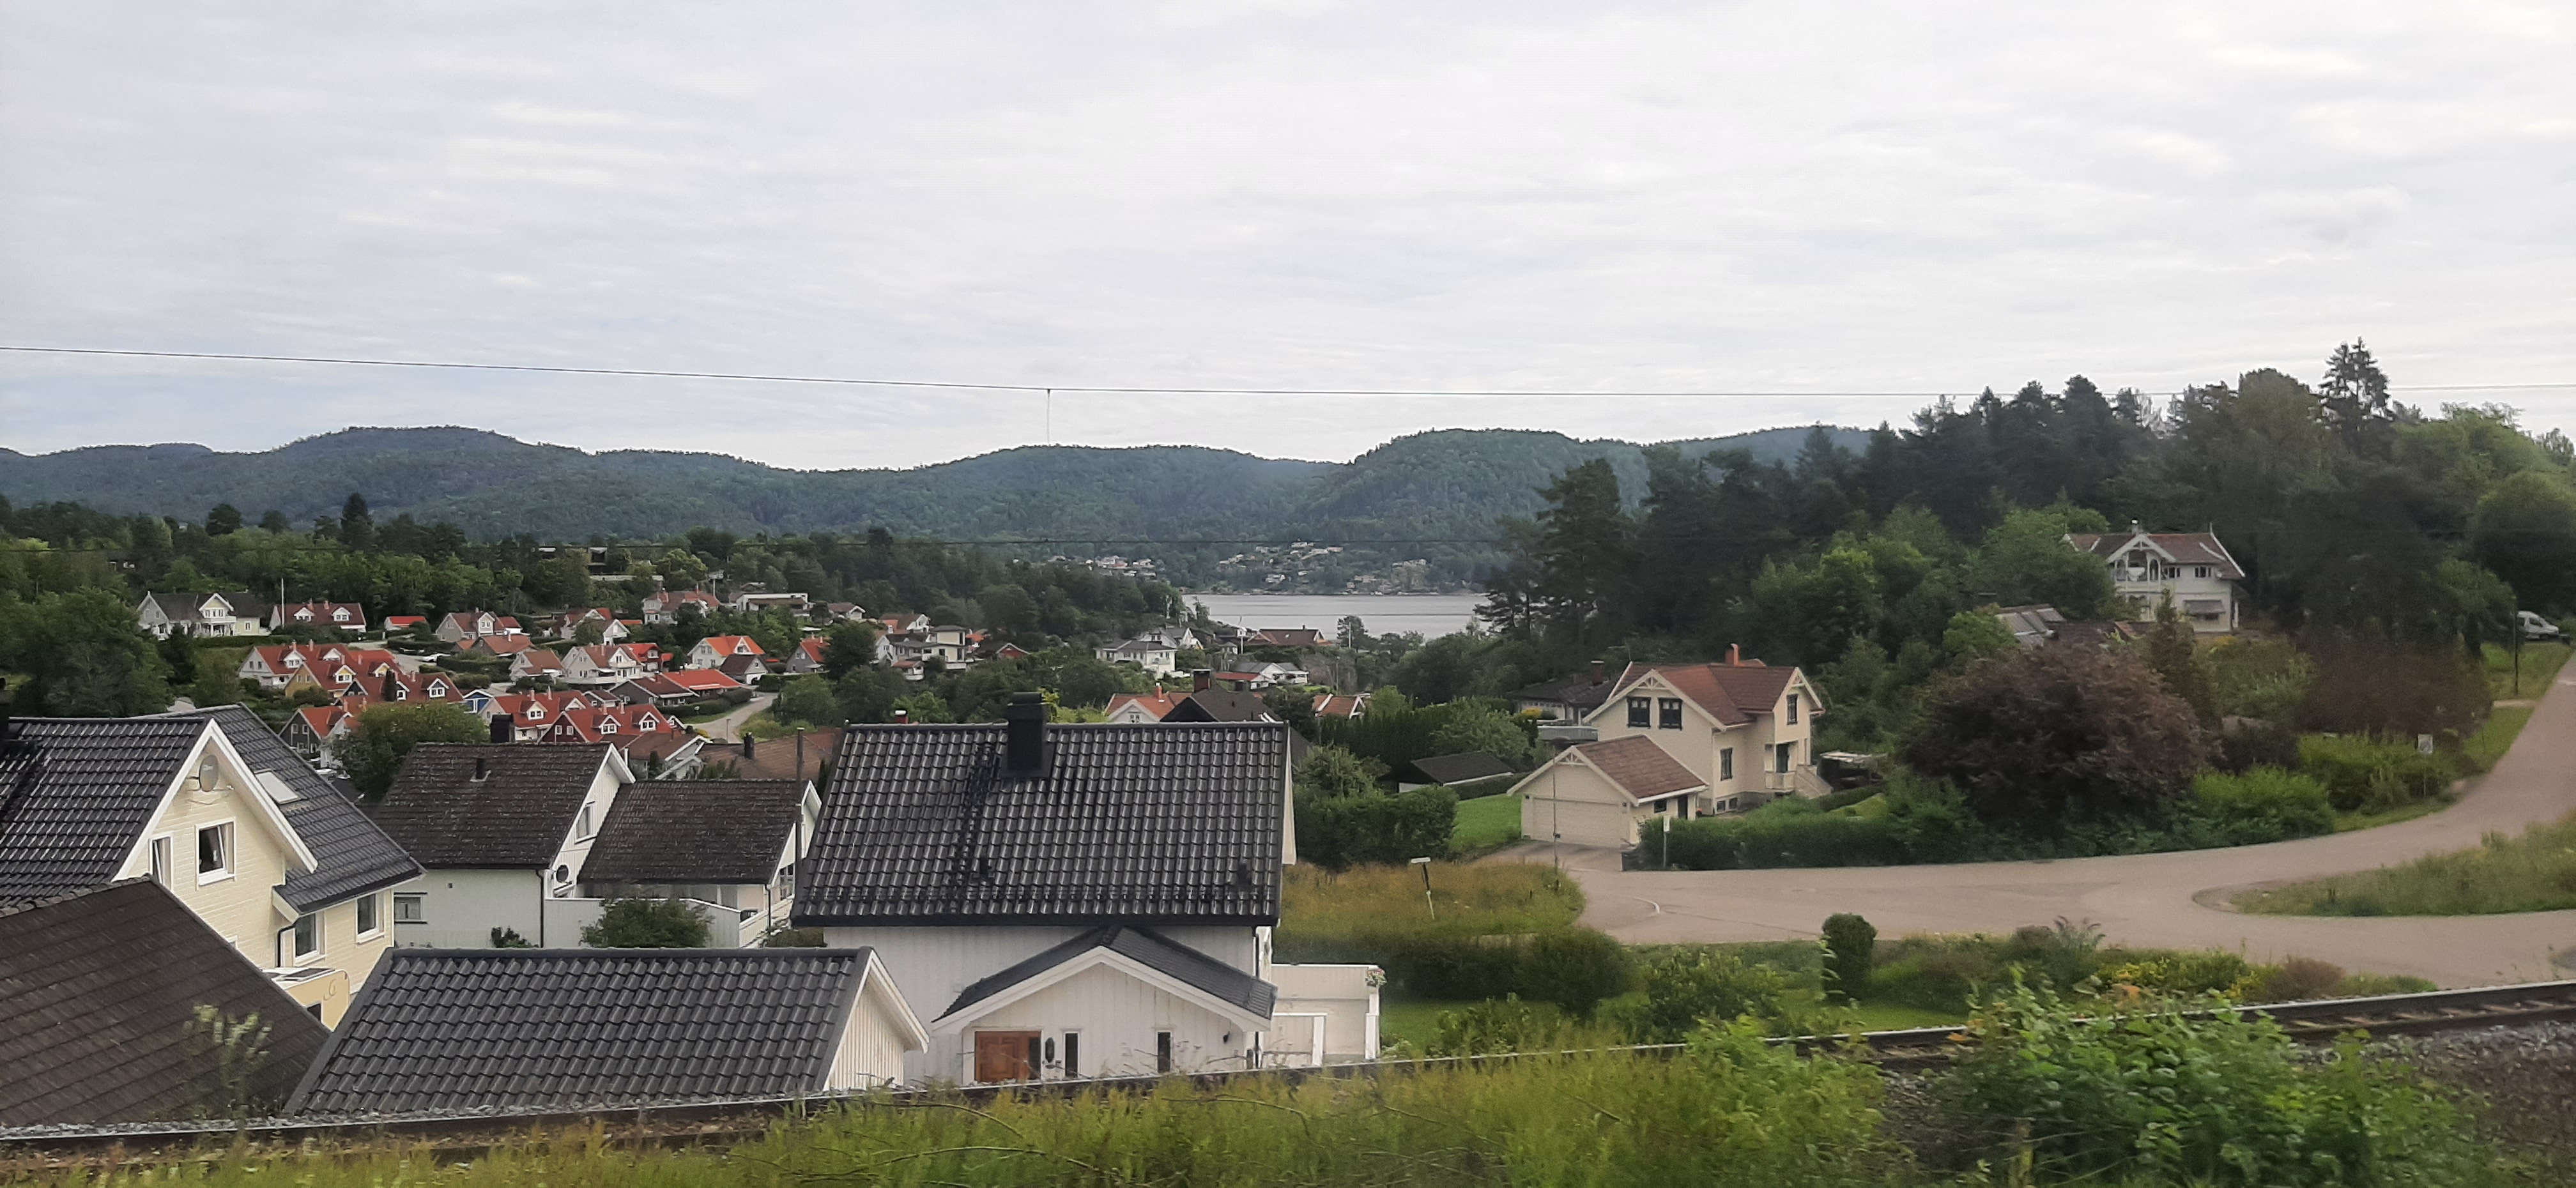
\includegraphics[width = 0.6\textwidth]{Plots/20230803_120917.jpg}
  \end{figure}
\end{frame}

\begin{frame}{Brief introduction to my PhD analysis}
  \begin{center}
    \Large{Status after 3 years:}
  \end{center}
  \vspace{0.1cm}
  \begin{enumerate}
    \setlength\itemsep{0.7em}
    \item{Final piece of my PhD analysis is coming together}
    \item{Just started on analysis of November 2022 TORCH testbeam data}
    \item{Will probably start writing PhD thesis next term}
  \end{enumerate}
  \vspace{-0.2cm}
  \begin{figure}
    \centering
    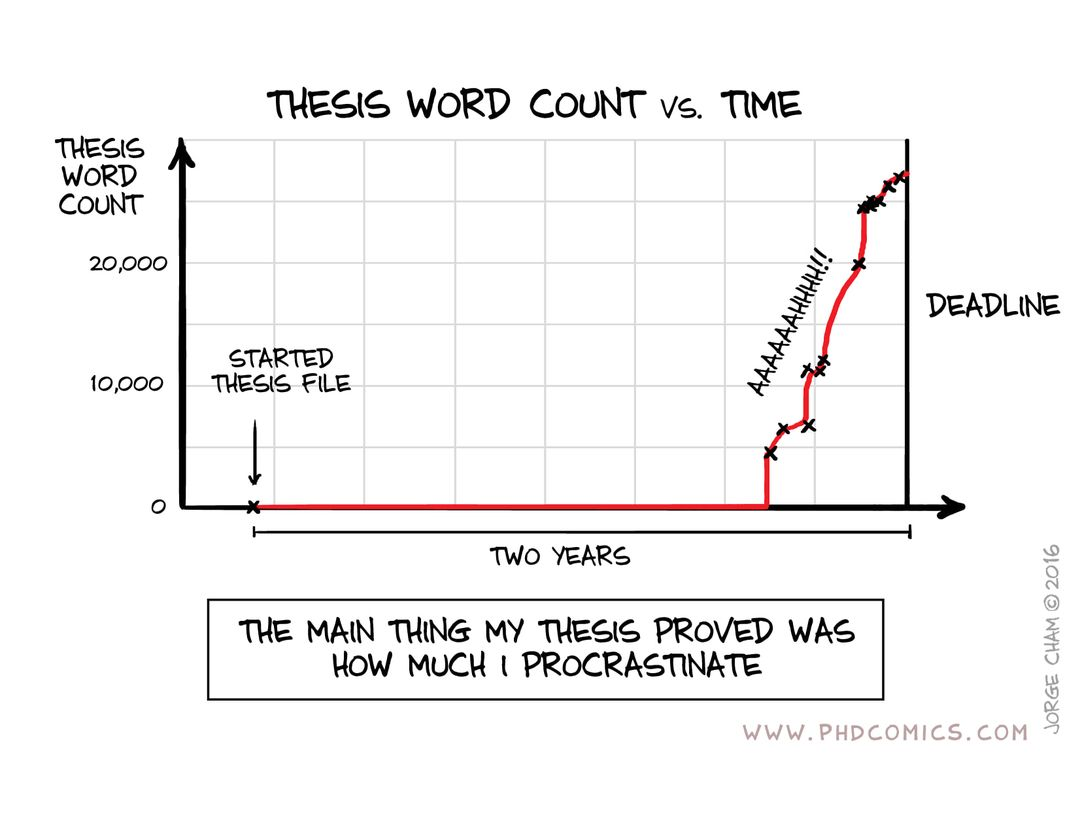
\includegraphics[width = 0.6\textwidth]{Plots/PhDThesisComic.jpg}
  \end{figure}
\end{frame}

\begin{frame}{Recap of LHCb analysis of $B^\pm\to[K^+K^-\pi^+\pi^-]_Dh^\pm$}
  \begin{center}
    LHCb paper: A study of CP violation in the decays $B^\pm\to[K^+K^-\pi^+\pi^-]_Dh^\pm$ $(h = K, \pi)$ and $B^\pm\to[\pi^+\pi^-\pi^+\pi^-]_Dh^\pm$
  \end{center}
  \vspace{0.1cm}
  \begin{itemize}
    \item{Binned model-dependent GGSZ analysis of $B^\pm\to[K^+K^-\pi^+\pi^-]_Dh^\pm$}
    \item{A $3\sigma$ tension: $\gamma = (116^{+12}_{-14})^\circ$}
  \end{itemize}
  \begin{figure}
    \centering
    \begin{subfigure}{0.4\textwidth}
      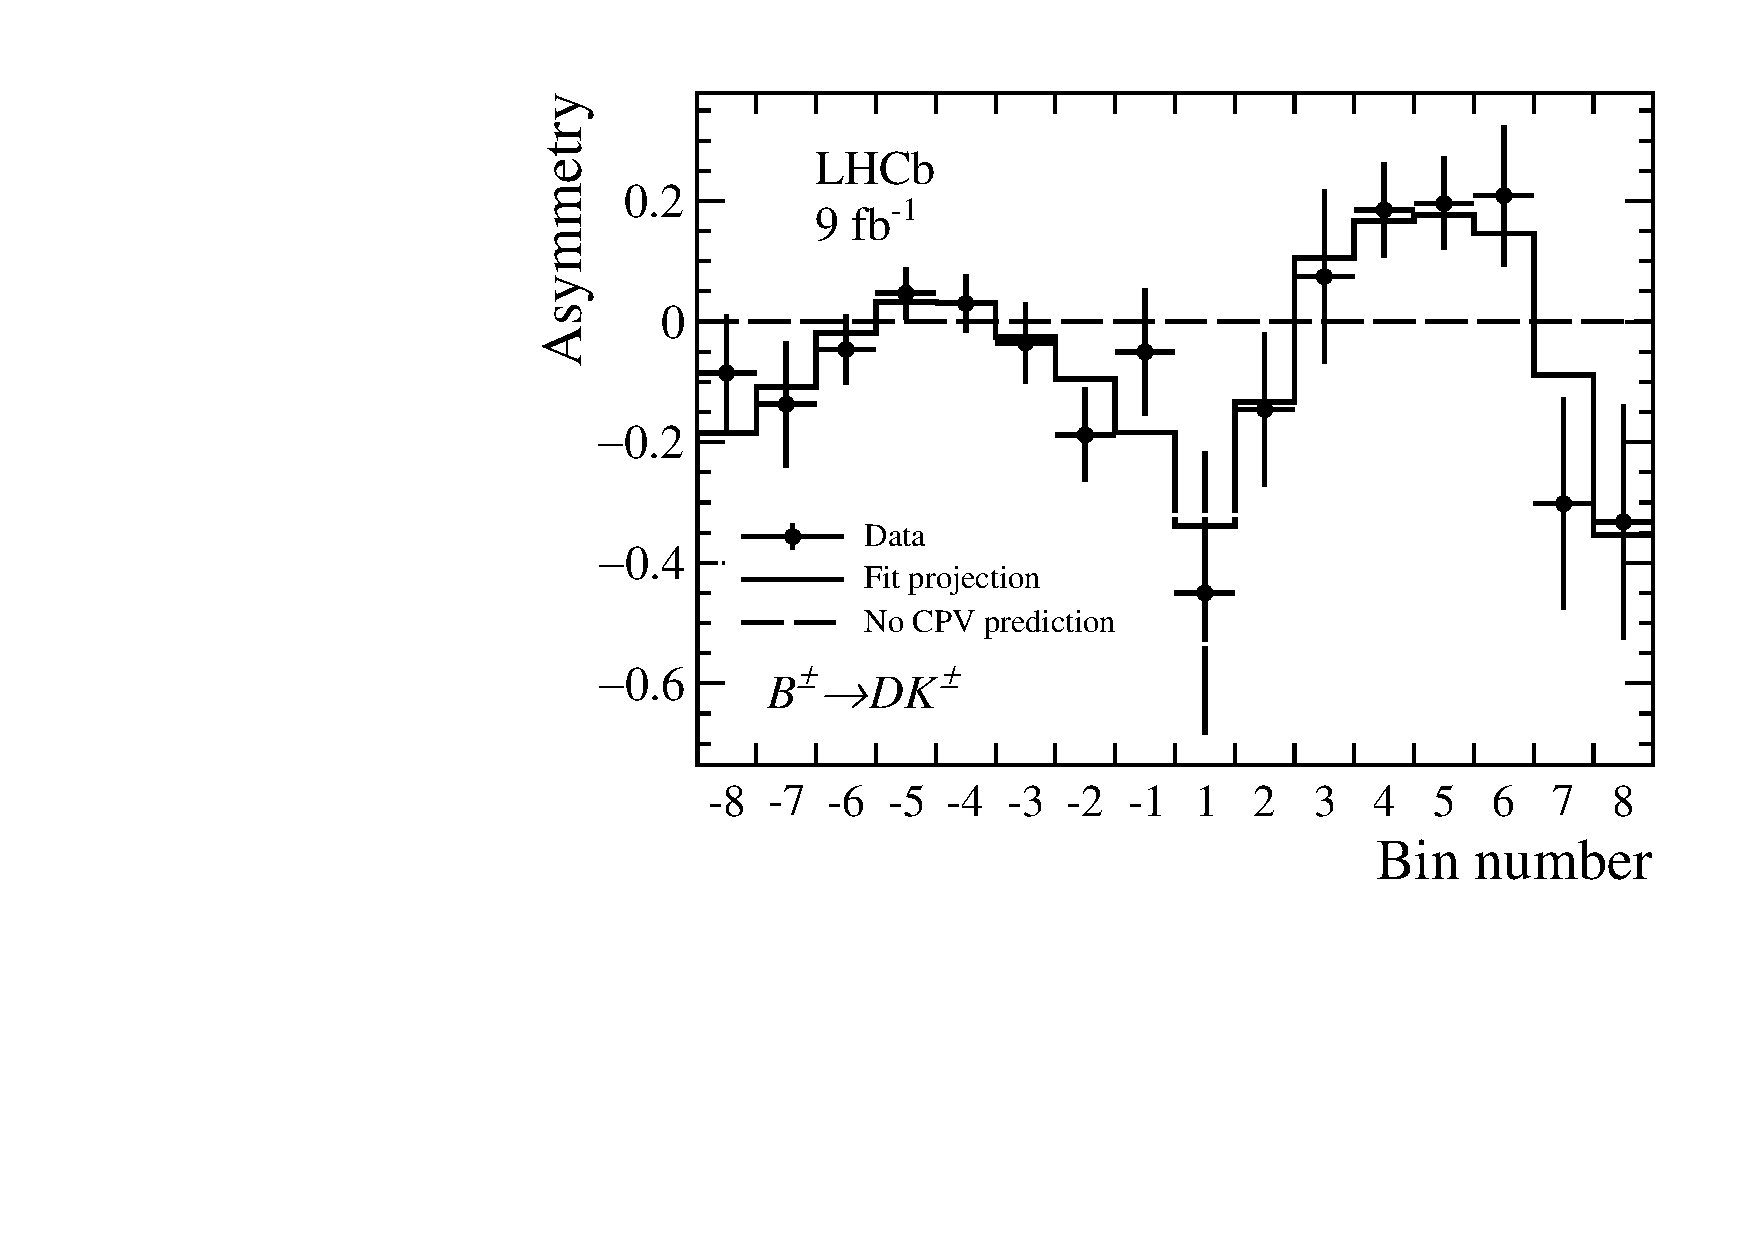
\includegraphics[width = 1.0\textwidth]{Plots/BinAsymmetries_dk.pdf}
    \end{subfigure}%
    \hspace{1cm}
    \begin{subfigure}{0.4\textwidth}
      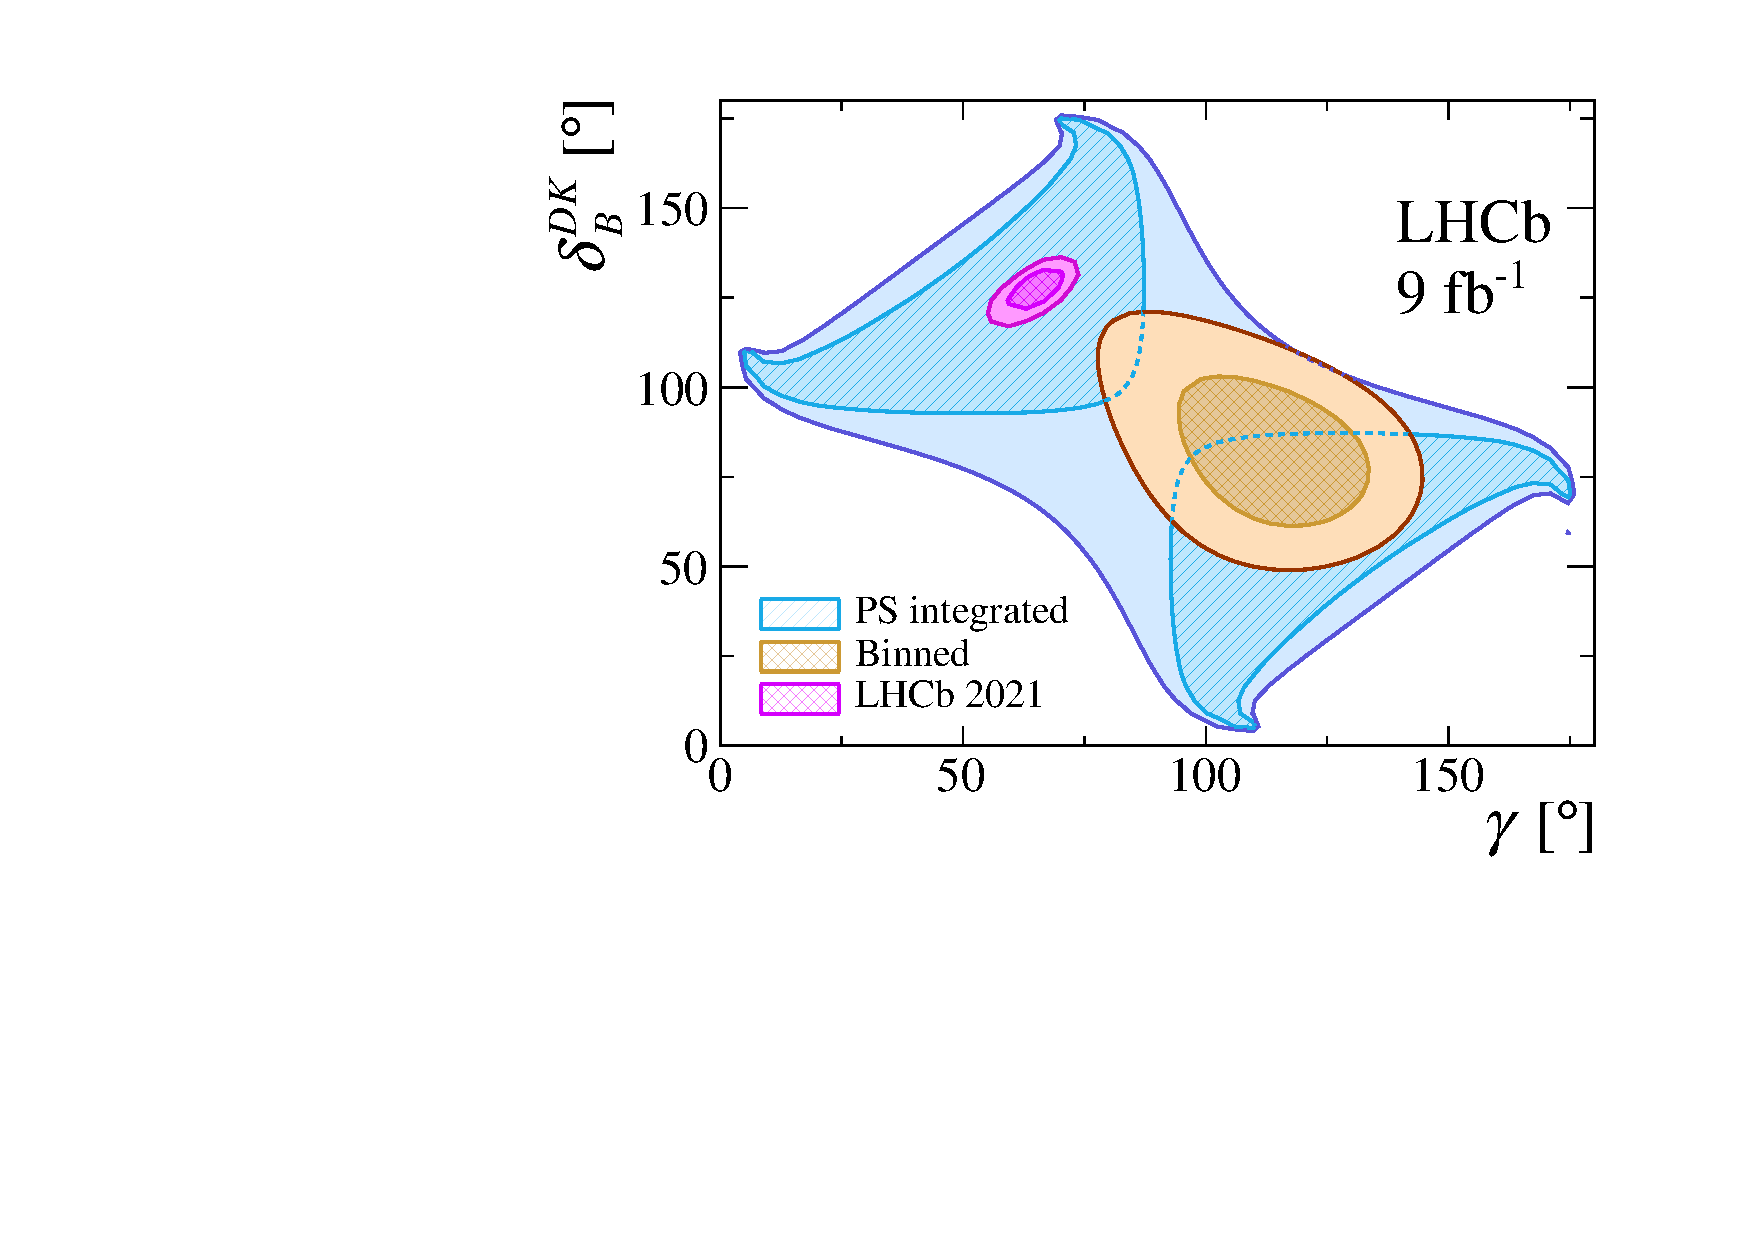
\includegraphics[width = 1.0\textwidth]{Plots/gammacharm_lhcb_KKpipi_GLW_KKpipi_GGSZ_lhcb_2020_beauty_and_charm_g_d_dk.pdf}
    \end{subfigure}
    \caption{Left: $B^\pm\to DK^\pm$ bin asymmetries. Right: Interpretation of $\gamma$}
  \end{figure}
\end{frame}

\begin{frame}{Recap of LHCb analysis of $B^\pm\to[K^+K^-\pi^+\pi^-]_Dh^\pm$}
  \begin{center}
    \Large{Why is there a $3\sigma$ tension?}
  \end{center}
  \begin{itemize}
    \setlength\itemsep{0.3em}
    \item{$D^0\to K^+K^-\pi^+\pi^-$ strong phases are from a model}
    \item{Model-independent inputs from BESIII are \underline{necessary}}
    \item{It's been challenge to convince reviewers that $\gamma$ is \underline{model dependent}:}
  \end{itemize}
  \vspace{0.5cm}
  \white{`` \textit{If you plan to keep the model-dependent value of gamma in the paper, the interpretation part should contain more discussion on the model dependence.}'' - EPJC referee 1} \\~\\
  \white{``\textit{A general comment is that in (7 !!) different places [Abstract, Introduction (page 1)...] it is mentioned the same message: that the analysis is model-dependent...}'' - EPJC referee 2}
\end{frame}

\begin{frame}{Recap of LHCb analysis of $B^\pm\to[K^+K^-\pi^+\pi^-]_Dh^\pm$}
  \begin{center}
    \Large{Why is there a $3\sigma$ tension?}
  \end{center}
  \begin{itemize}
    \setlength\itemsep{0.3em}
    \item{$D^0\to K^+K^-\pi^+\pi^-$ strong phases are from a model}
    \item{Model-independent inputs from BESIII are \underline{necessary}}
    \item{It's been challenge to convince reviewers that $\gamma$ is \underline{model dependent}:}
  \end{itemize}
  \vspace{0.5cm}
  `` \textit{If you plan to keep the model-dependent value of gamma in the paper, the interpretation part should contain more discussion on the model dependence.}'' - EPJC referee 1 \\~\\
  \white{``\textit{A general comment is that in (7 !!) different places [Abstract, Introduction (page 1)...] it is mentioned the same message: that the analysis is model-dependent...}'' - EPJC referee 2}
\end{frame}

\begin{frame}{Recap of LHCb analysis of $B^\pm\to[K^+K^-\pi^+\pi^-]_Dh^\pm$}
  \begin{center}
    \Large{Why is there a $3\sigma$ tension?}
  \end{center}
  \begin{itemize}
    \setlength\itemsep{0.3em}
    \item{$D^0\to K^+K^-\pi^+\pi^-$ strong phases are from a model}
    \item{Model-independent inputs from BESIII are \underline{necessary}}
    \item{It's been challenge to convince reviewers that $\gamma$ is \underline{model dependent}:}
  \end{itemize}
  \vspace{0.5cm}
  `` \textit{If you plan to keep the model-dependent value of gamma in the paper, the interpretation part should contain more discussion on the model dependence.}'' - EPJC referee 1 \\~\\
  ``\textit{A general comment is that in (7 !!) different places [Abstract, Introduction (page 1)...] it is mentioned the same message: that the analysis is model-dependent...}'' - EPJC referee 2
\end{frame}

\section{BESIII strong-phase measurement}

\begin{frame}{Brief summary of formalism}
  \begin{itemize}
    \setlength\itemsep{0.5em}
    \item{Identical formalism to BPGGSZ analyses with $D^0\to K_S^0h^+h^-$}
    \item{Split events into bins of phase space}
    \item{LHCb: Measure CP asymmetries in each bin}
    \item{BESIII: Measure the cosine (sine) of the strong-phase difference $c_i$ ($s_i$)}
  \end{itemize}
  \begin{figure}
    \centering
    \begin{subfigure}{0.37\textwidth}
      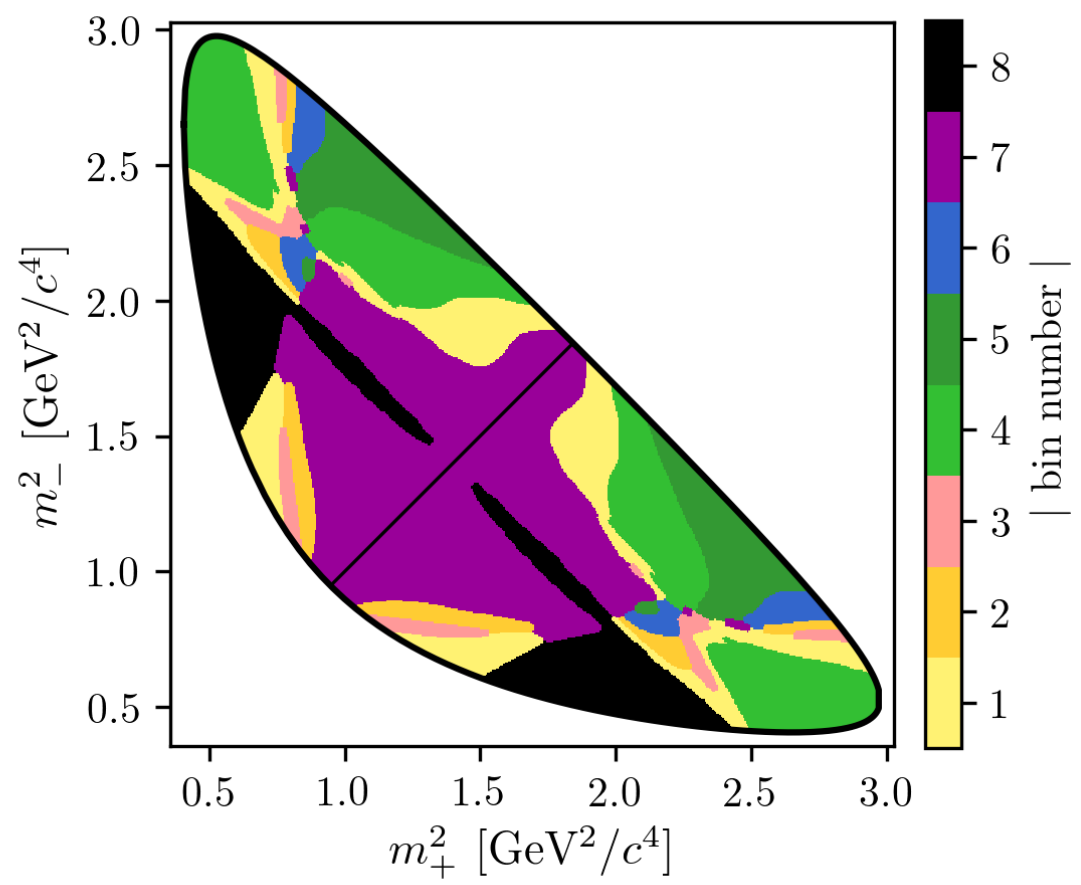
\includegraphics[width = 1.0\textwidth]{Plots/DalitzKSpipi.png}
    \end{subfigure}%
    \hspace{1cm}
    \begin{subfigure}{0.42\textwidth}
      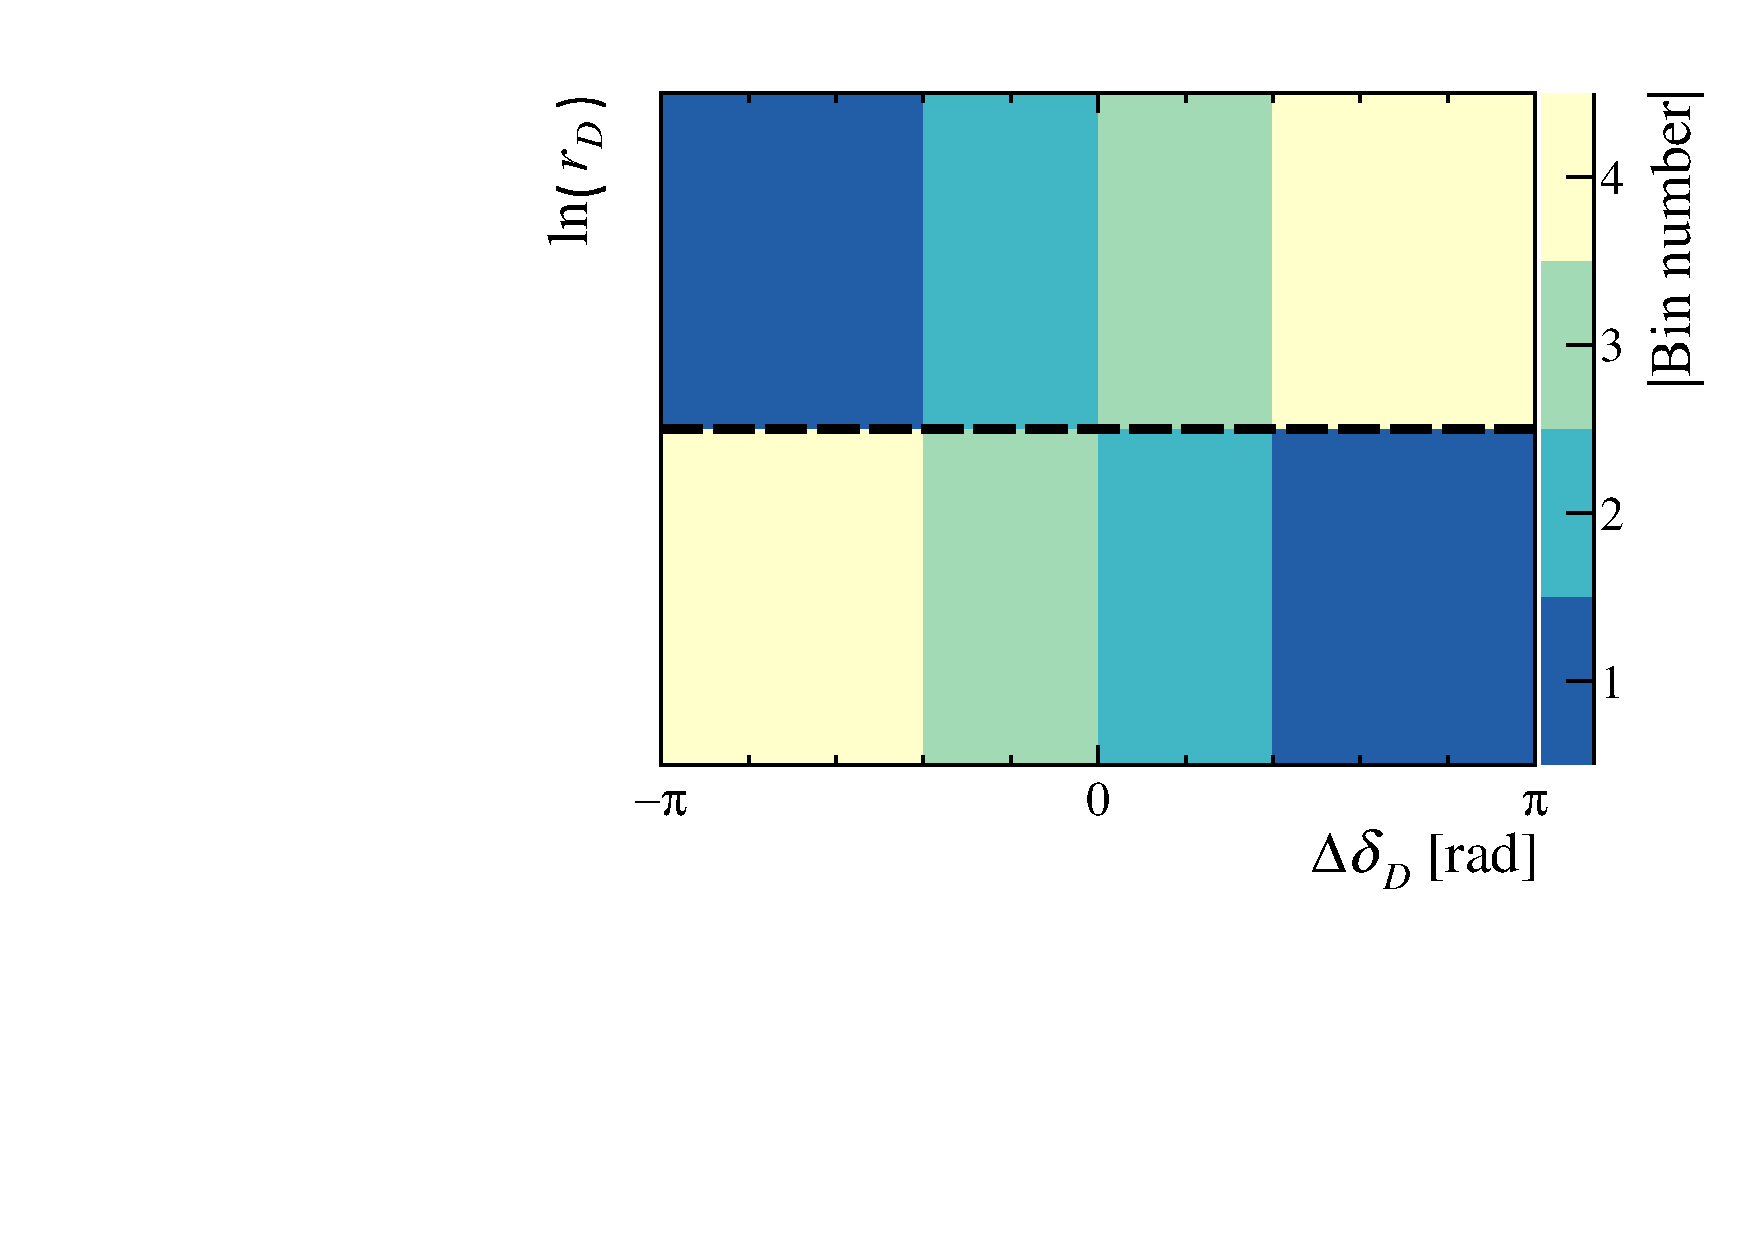
\includegraphics[width = 1.0\textwidth]{Plots/BinningSchemePlot_4Bins.pdf}
    \end{subfigure}
    \caption{Left: Binning scheme of $D^0\to K_S^0\pi^+\pi^-$, visualised on a Dalitz plot. Right: Analogous binning scheme for $D^0\to K^+K^-\pi^+\pi^-$, where the 5D phase space is projected onto the model-predicted $\delta_D$ and $r_D$.}
  \end{figure}
\end{frame}

\begin{frame}{BESII $c_i$ and $s_i$ results}
  \begin{center}
    \Large{How to measure $c_i$ and $s_i$? Sneha already introduced BESIII in last week's seminar!}
  \end{center}
  \begin{enumerate}
    \setlength\itemsep{1.0em}
    \item{Measure the double-tag yields}
    \item{Tags with different CP content can enhance/suppress yields}
    \item{Infer $c_i$ and $s_i$ in a large simultaneous fit of all tags}
  \end{enumerate}
  \begin{figure}
    \centering
    \begin{subfigure}{0.37\textwidth}
      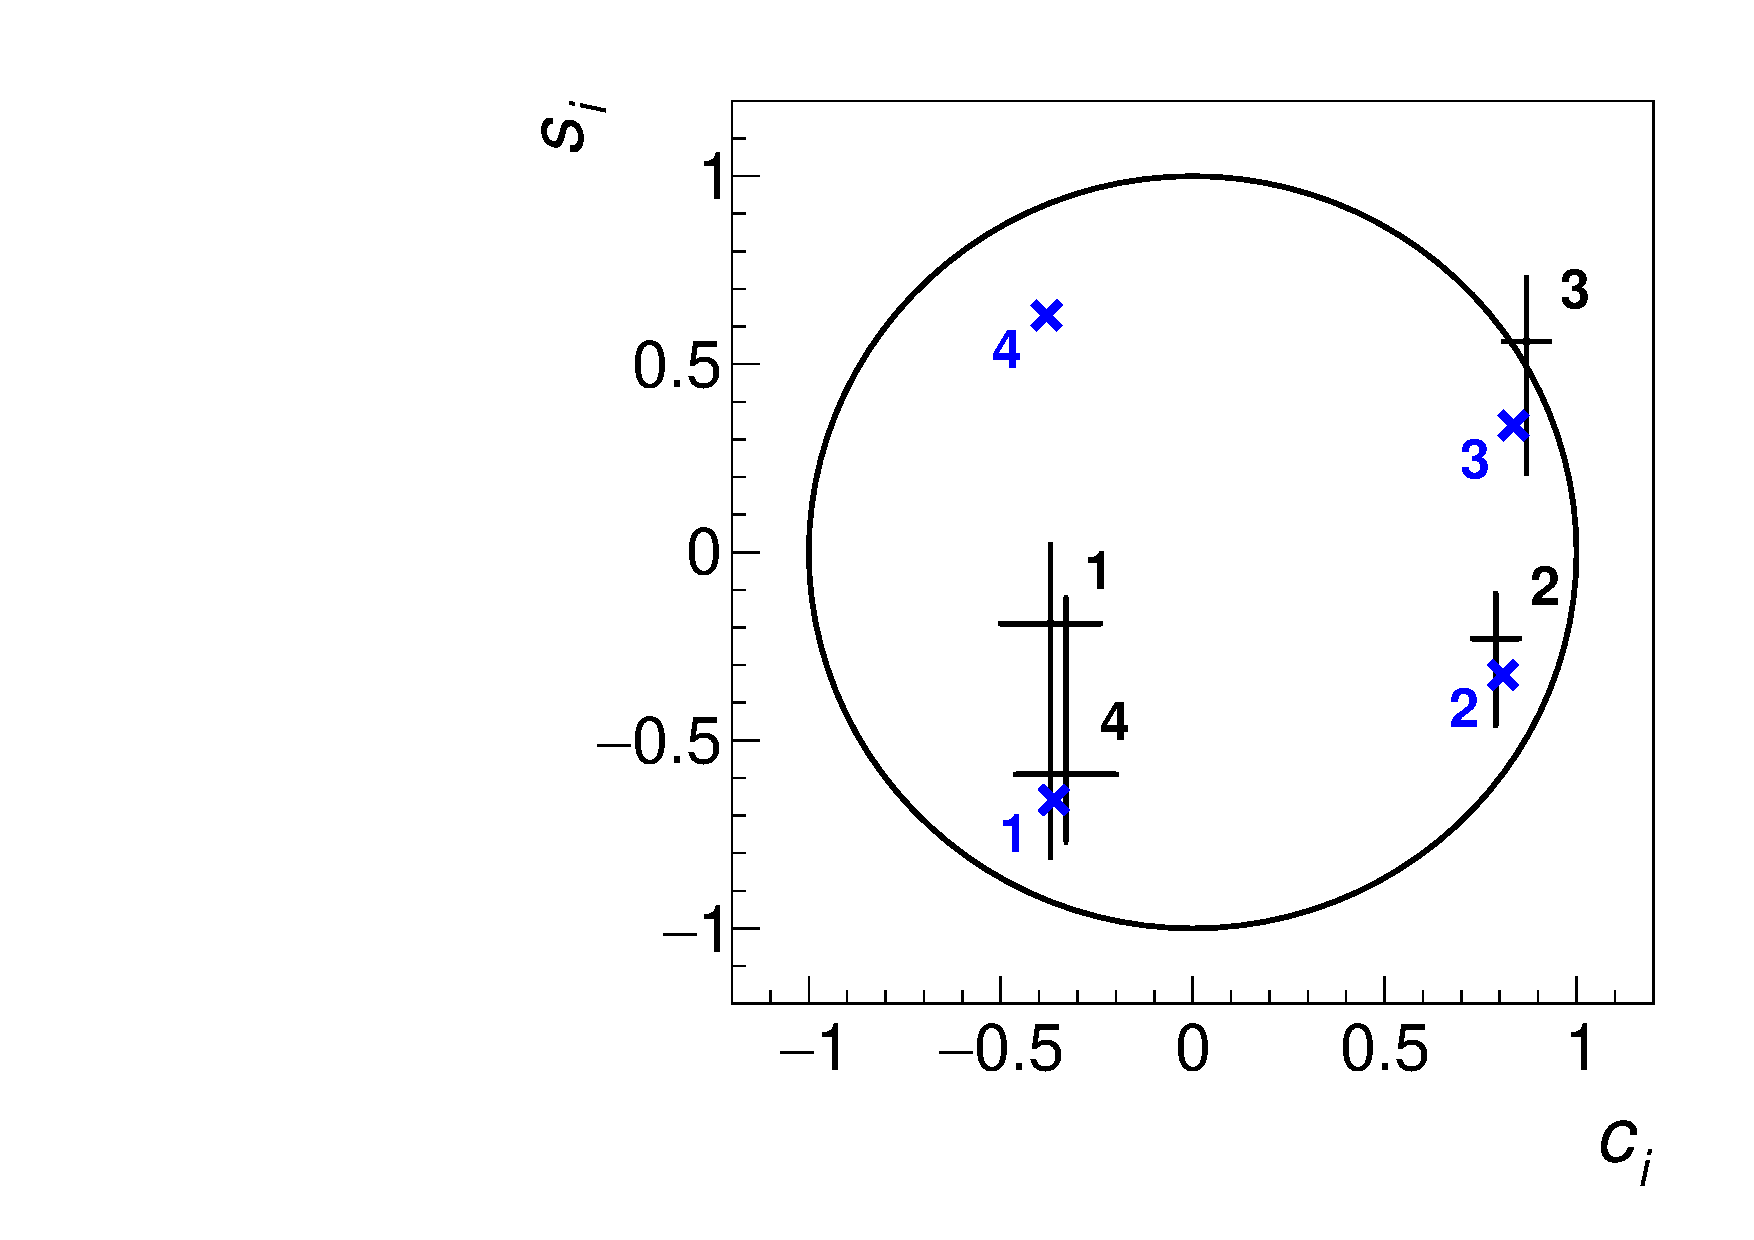
\includegraphics[width = 1.0\textwidth]{Plots/cisi_FitResults_Model.pdf}
    \end{subfigure}%
    \hspace{1cm}
    \begin{subfigure}{0.30\textwidth}
      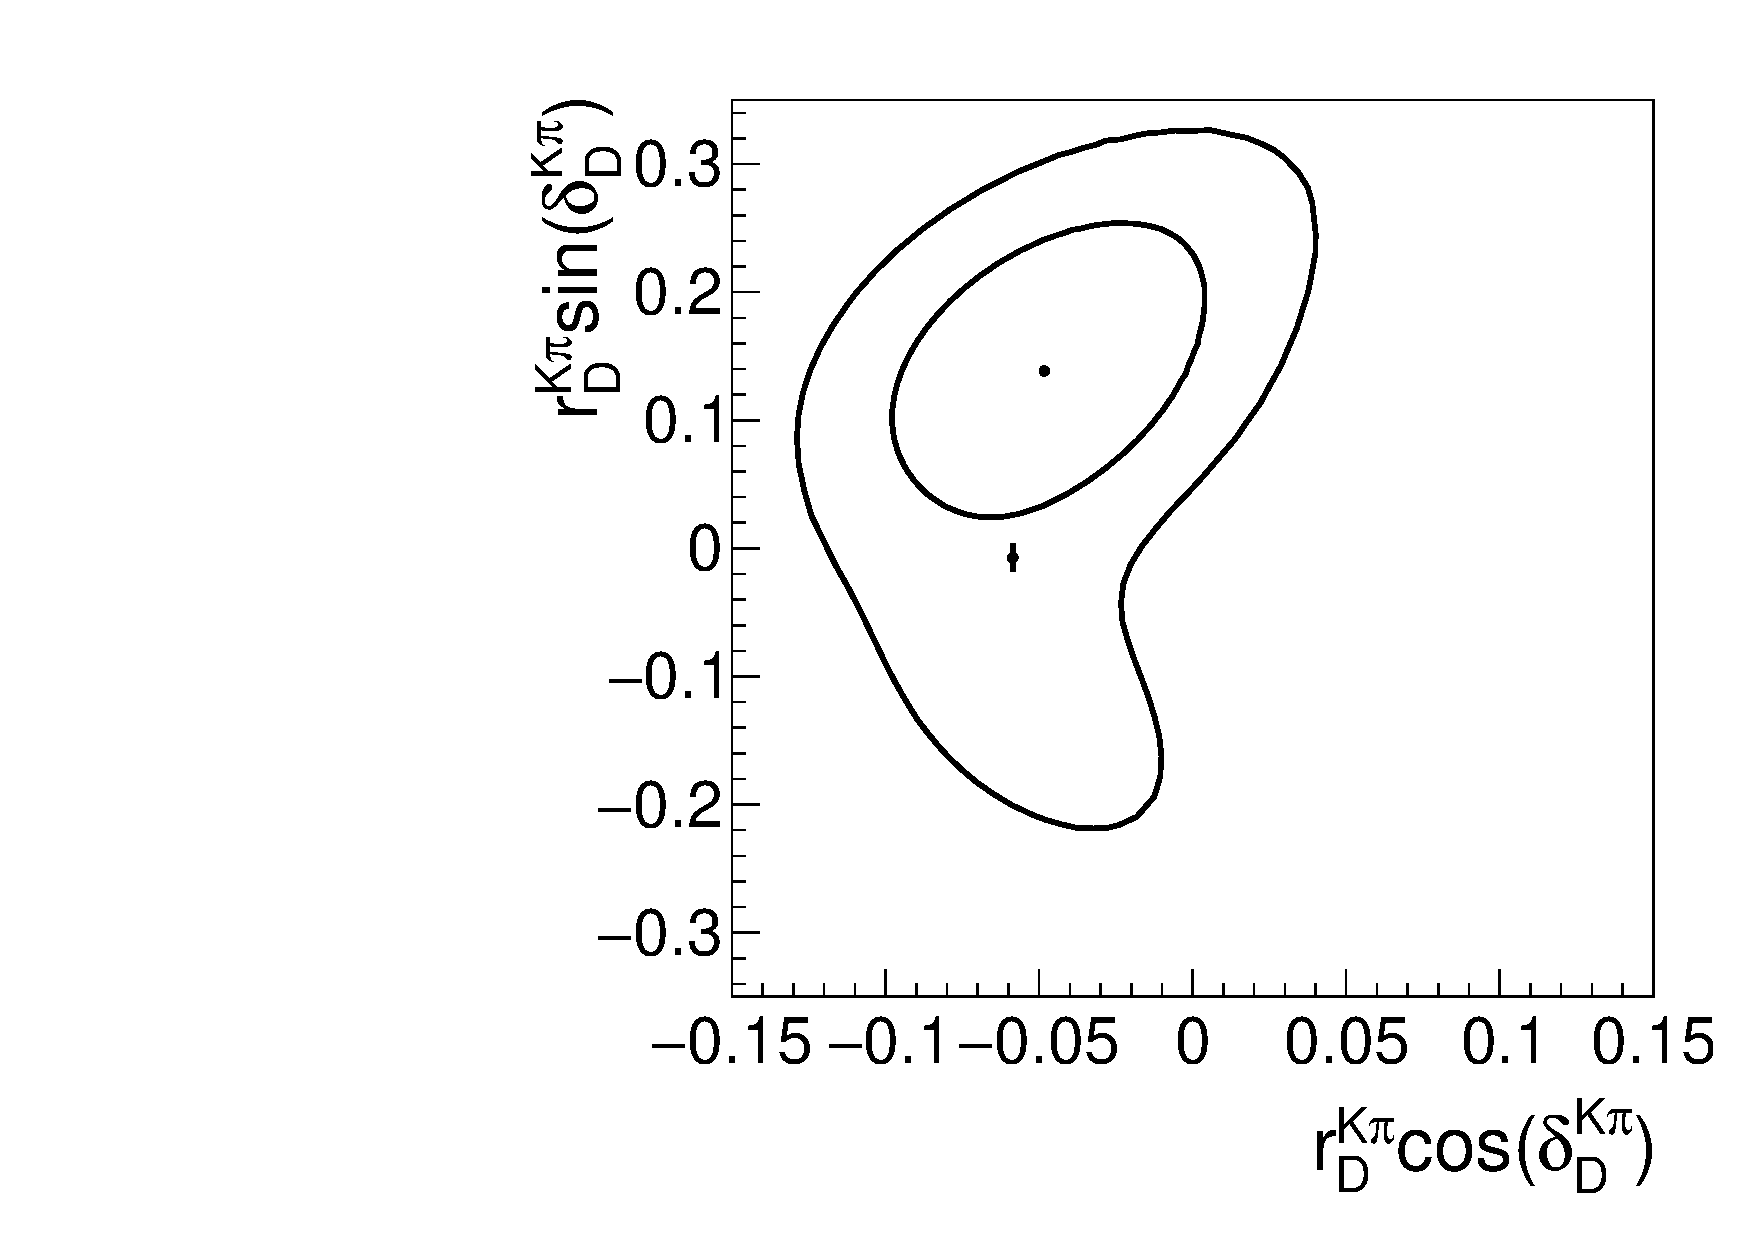
\includegraphics[width = 1.0\textwidth]{Plots/Contour_DeltaKpi.pdf}
    \end{subfigure}
    \caption{Left: Measurement of $c_i$ vs $s_i$. Right: Measurement of $\delta_D^{K\pi}$}
  \end{figure}
\end{frame}

\begin{frame}{Double tag fit of $KK\pi\pi$ vs $K\pi$}
  \begin{figure}
    \centering
    \begin{subfigure}{0.5\textwidth}
      \centering
      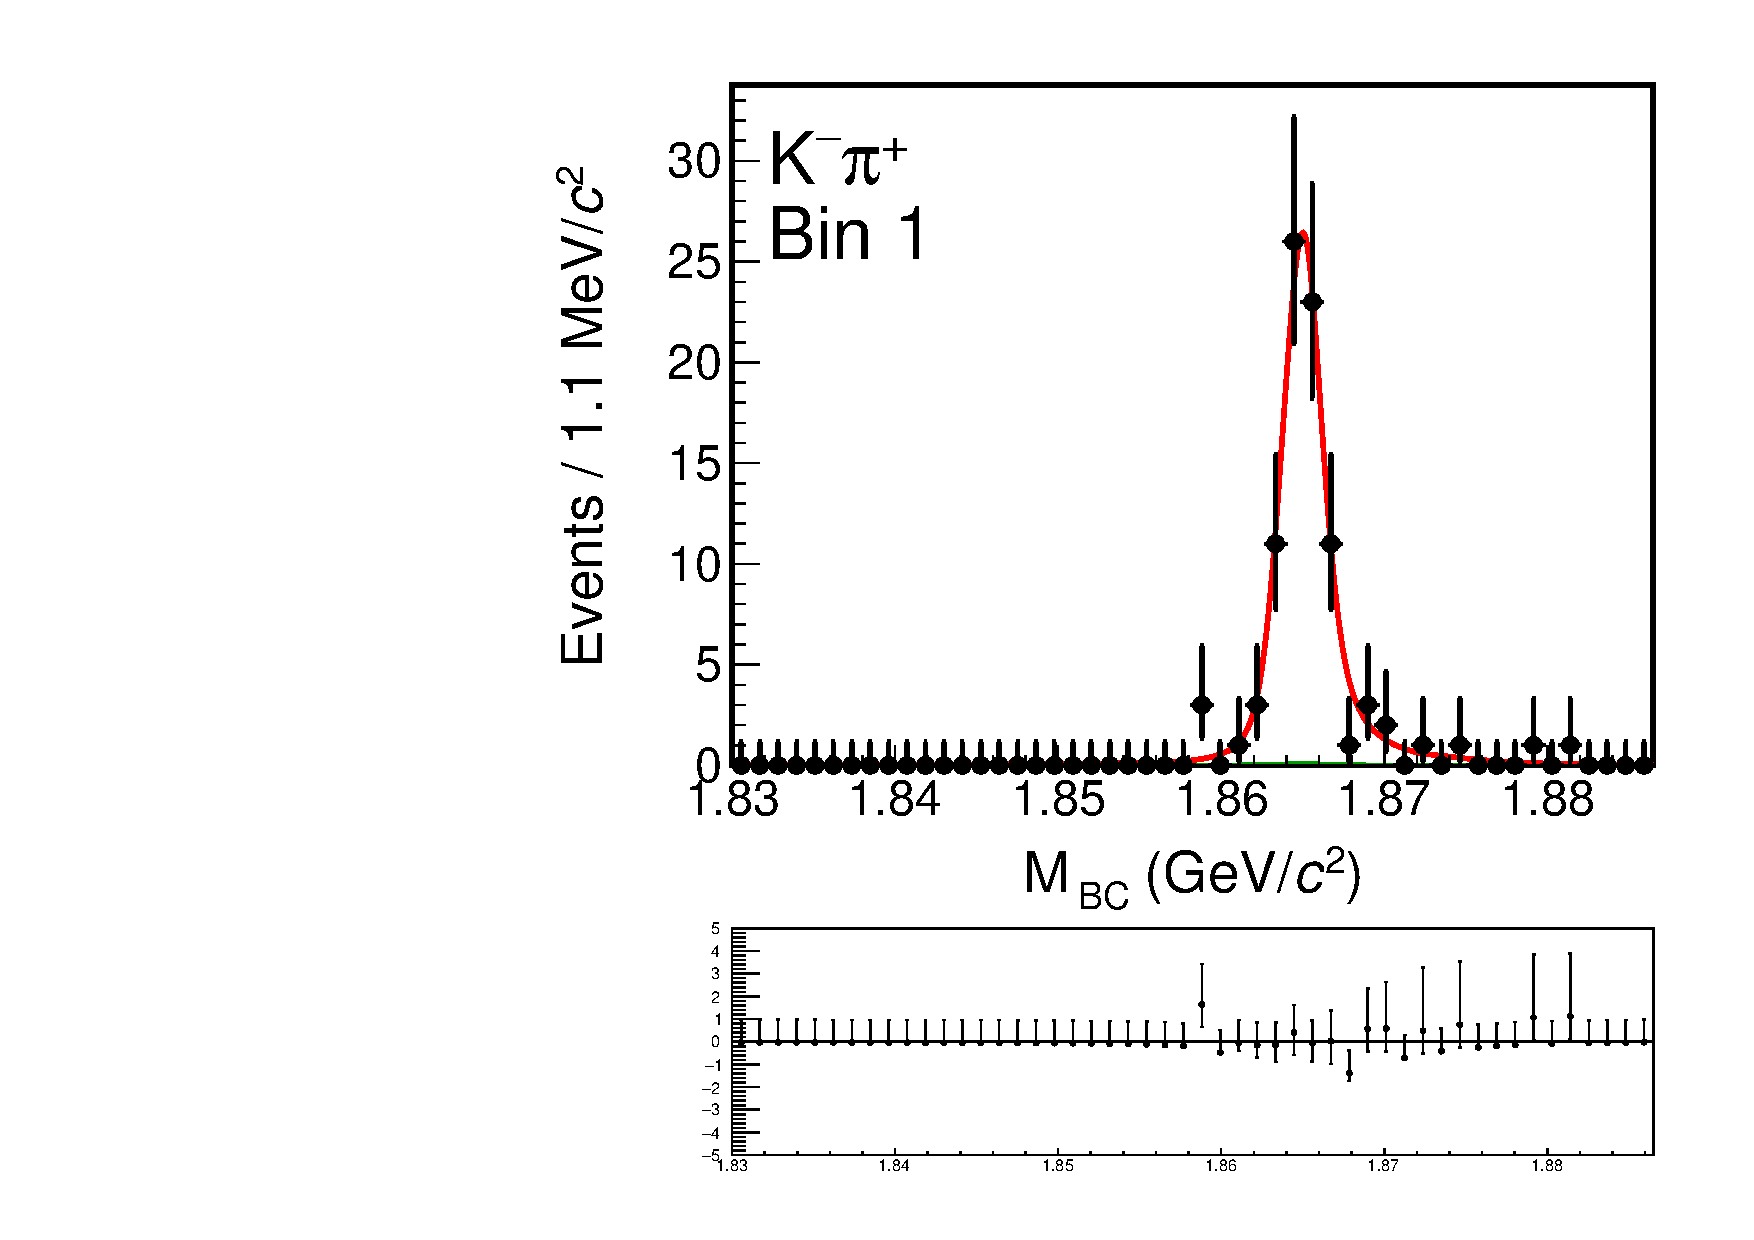
\includegraphics[width=0.75\textwidth,trim={0 5cm 0 0},clip=true]{Plots/DoubleTagYield_DoubleTag_Flavour_KKpipi_vs_Kpi_SignalBinP1_TagBin0.pdf}
      \caption{Bin $1$ yield: $84.5_{-9.1}^{+9.8}$}
    \end{subfigure}%
    \begin{subfigure}{0.5\textwidth}
      \centering
      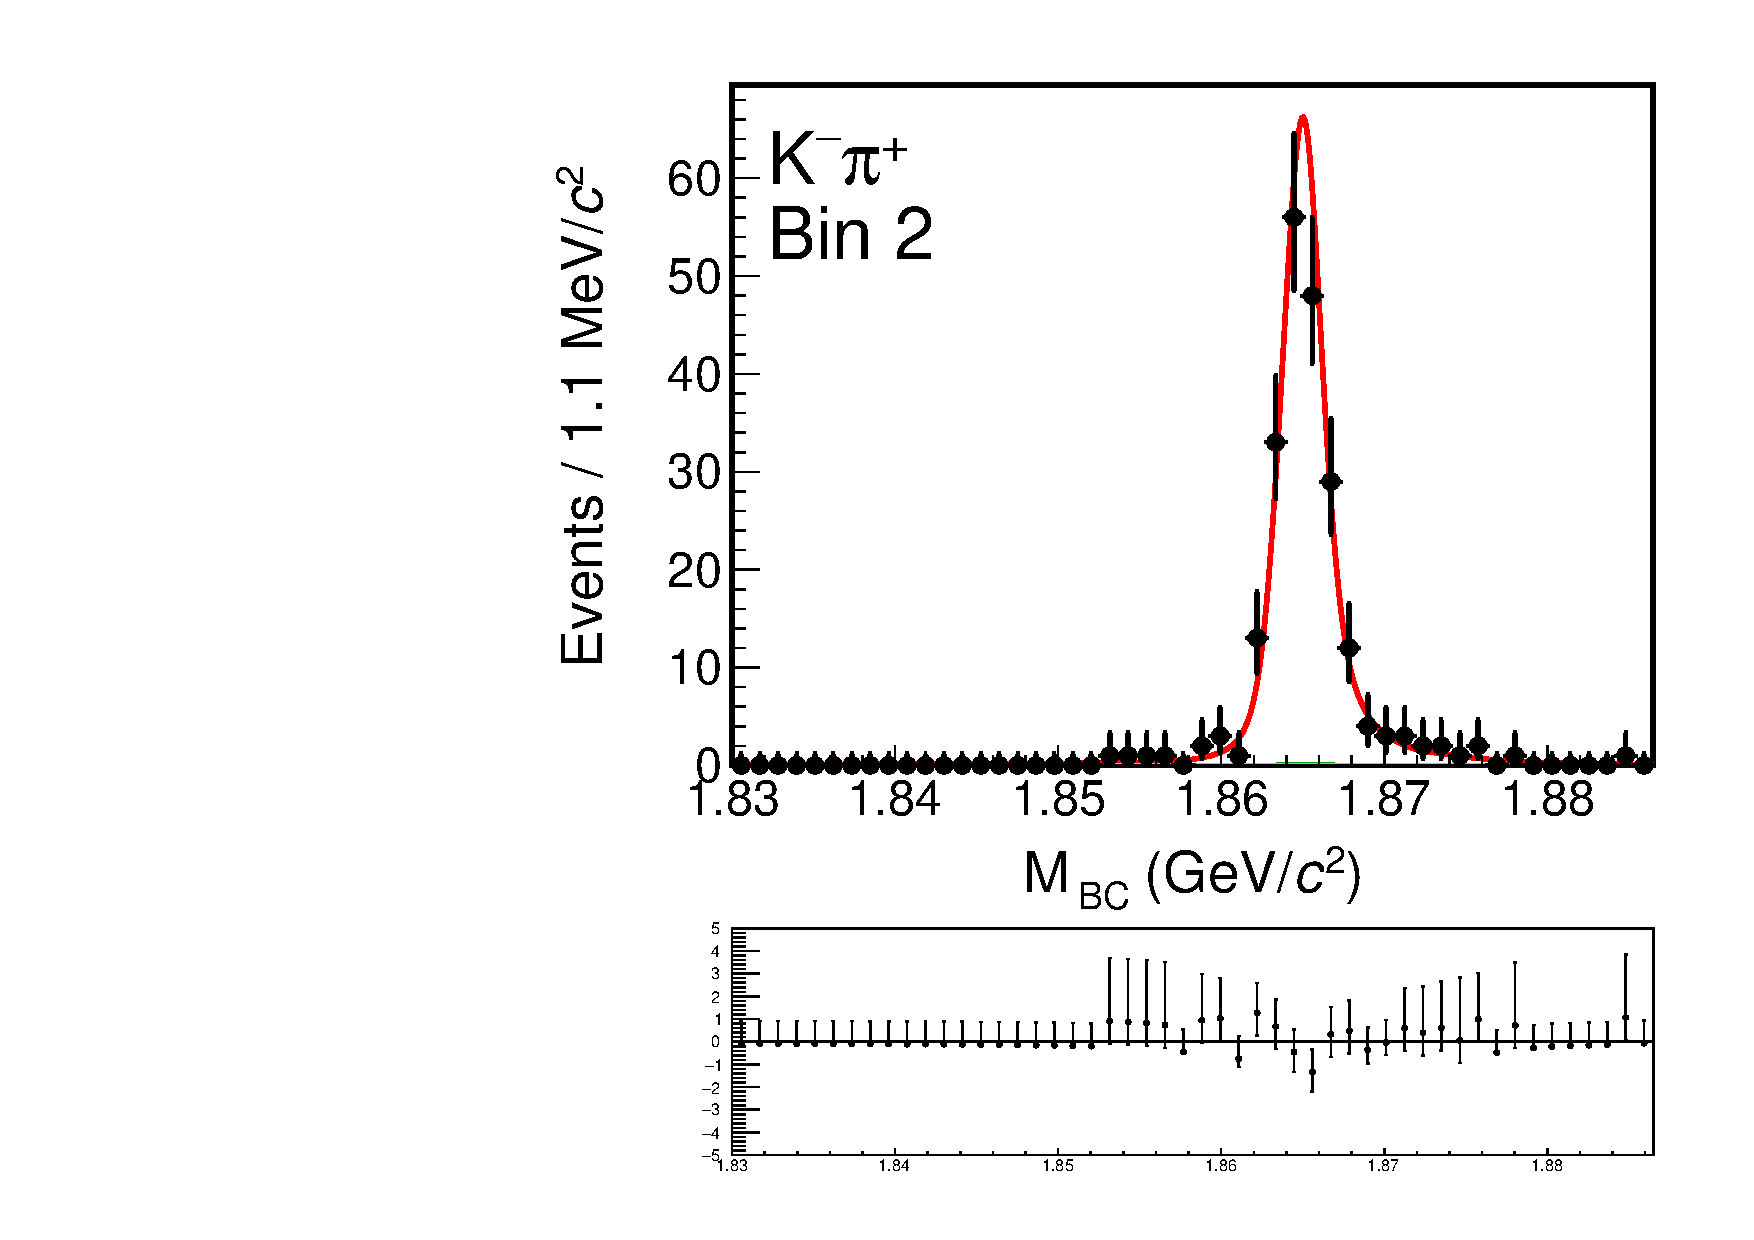
\includegraphics[width=0.75\textwidth,trim={0 5cm 0 0},clip=true]{Plots/DoubleTagYield_DoubleTag_Flavour_KKpipi_vs_Kpi_SignalBinP2_TagBin0.pdf}
      \caption{Bin $2$ yield: $211.2_{-14.8}^{+15.4}$}
    \end{subfigure}
    \begin{subfigure}{0.5\textwidth}
      \centering
      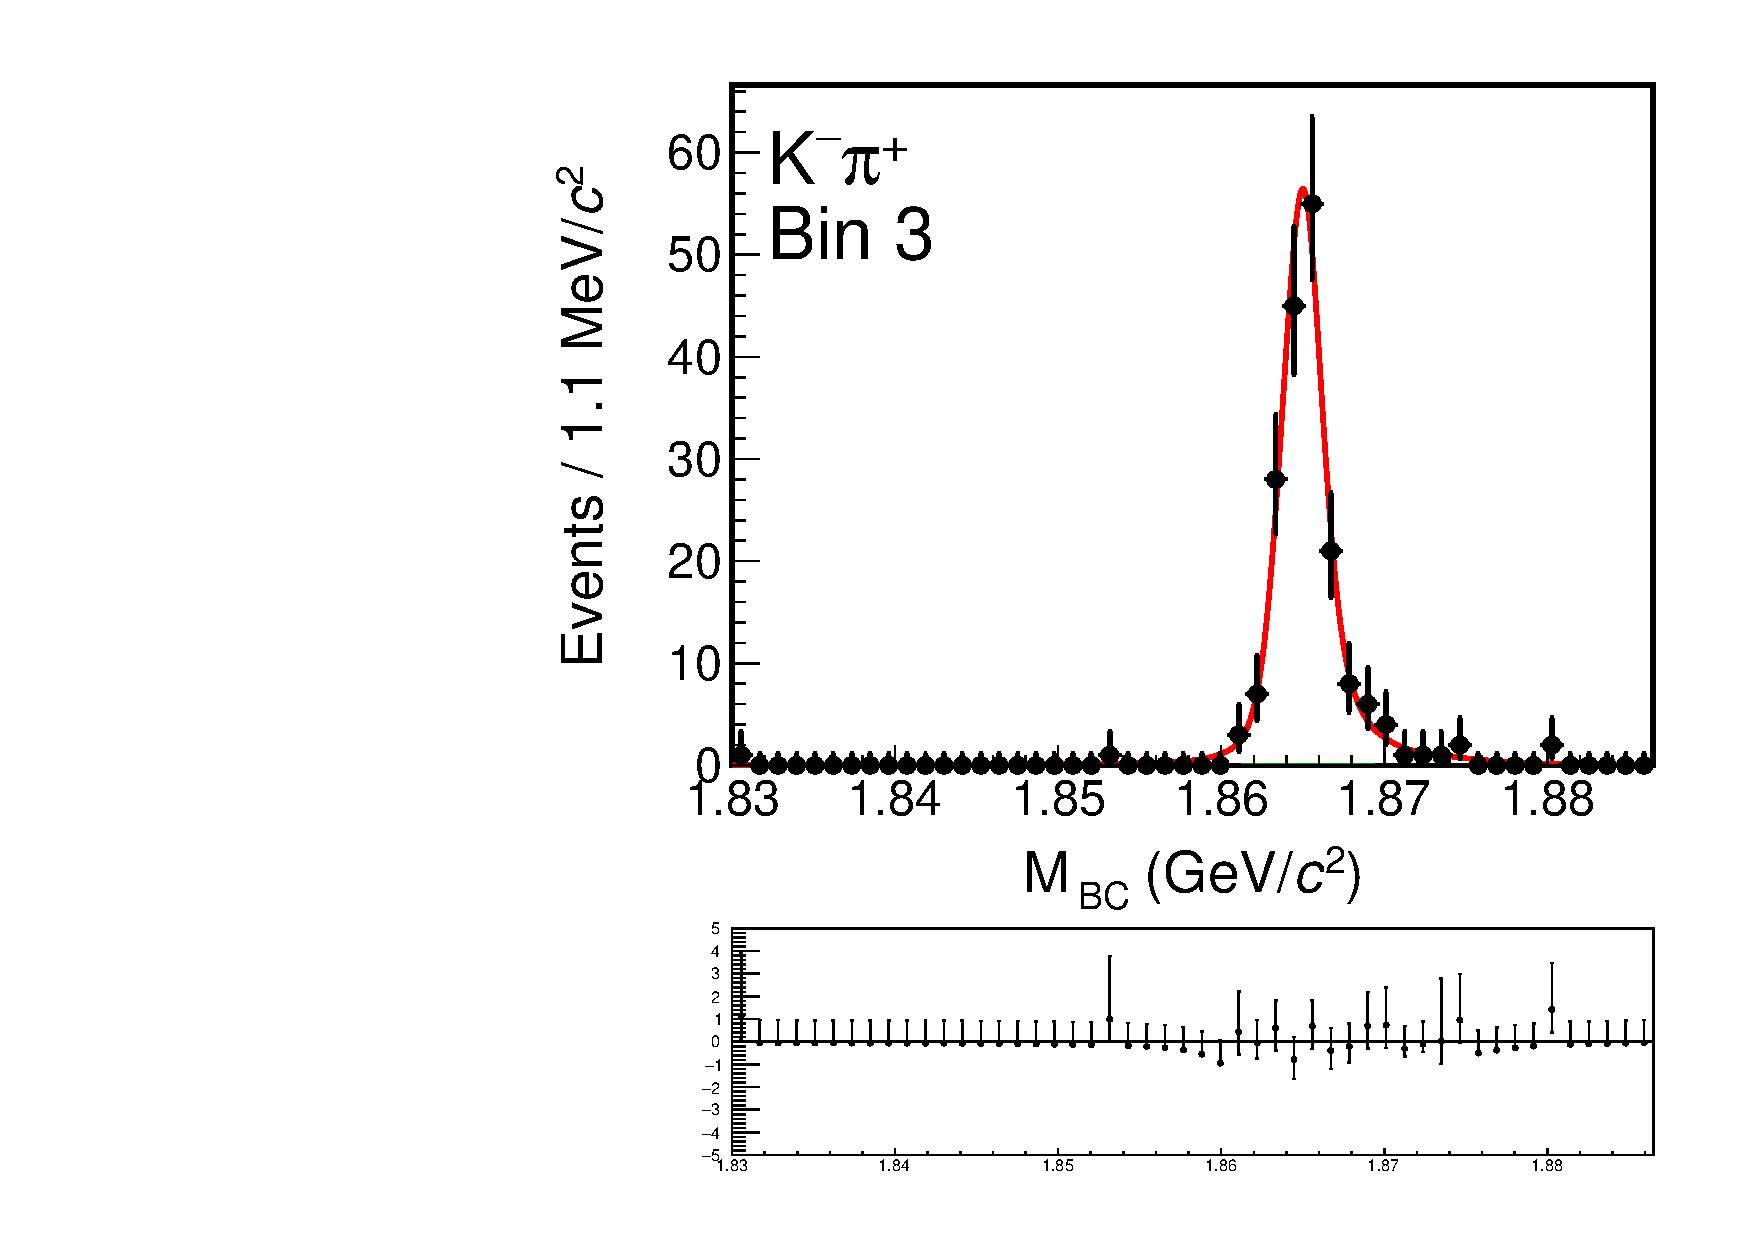
\includegraphics[width=0.75\textwidth,trim={0 5cm 0 0},clip=true]{Plots/DoubleTagYield_DoubleTag_Flavour_KKpipi_vs_Kpi_SignalBinP3_TagBin0.pdf}
      \caption{Bin $3$ yield: $181.0_{-13.3}^{+14.0}$}
    \end{subfigure}%
    \begin{subfigure}{0.5\textwidth}
      \centering
      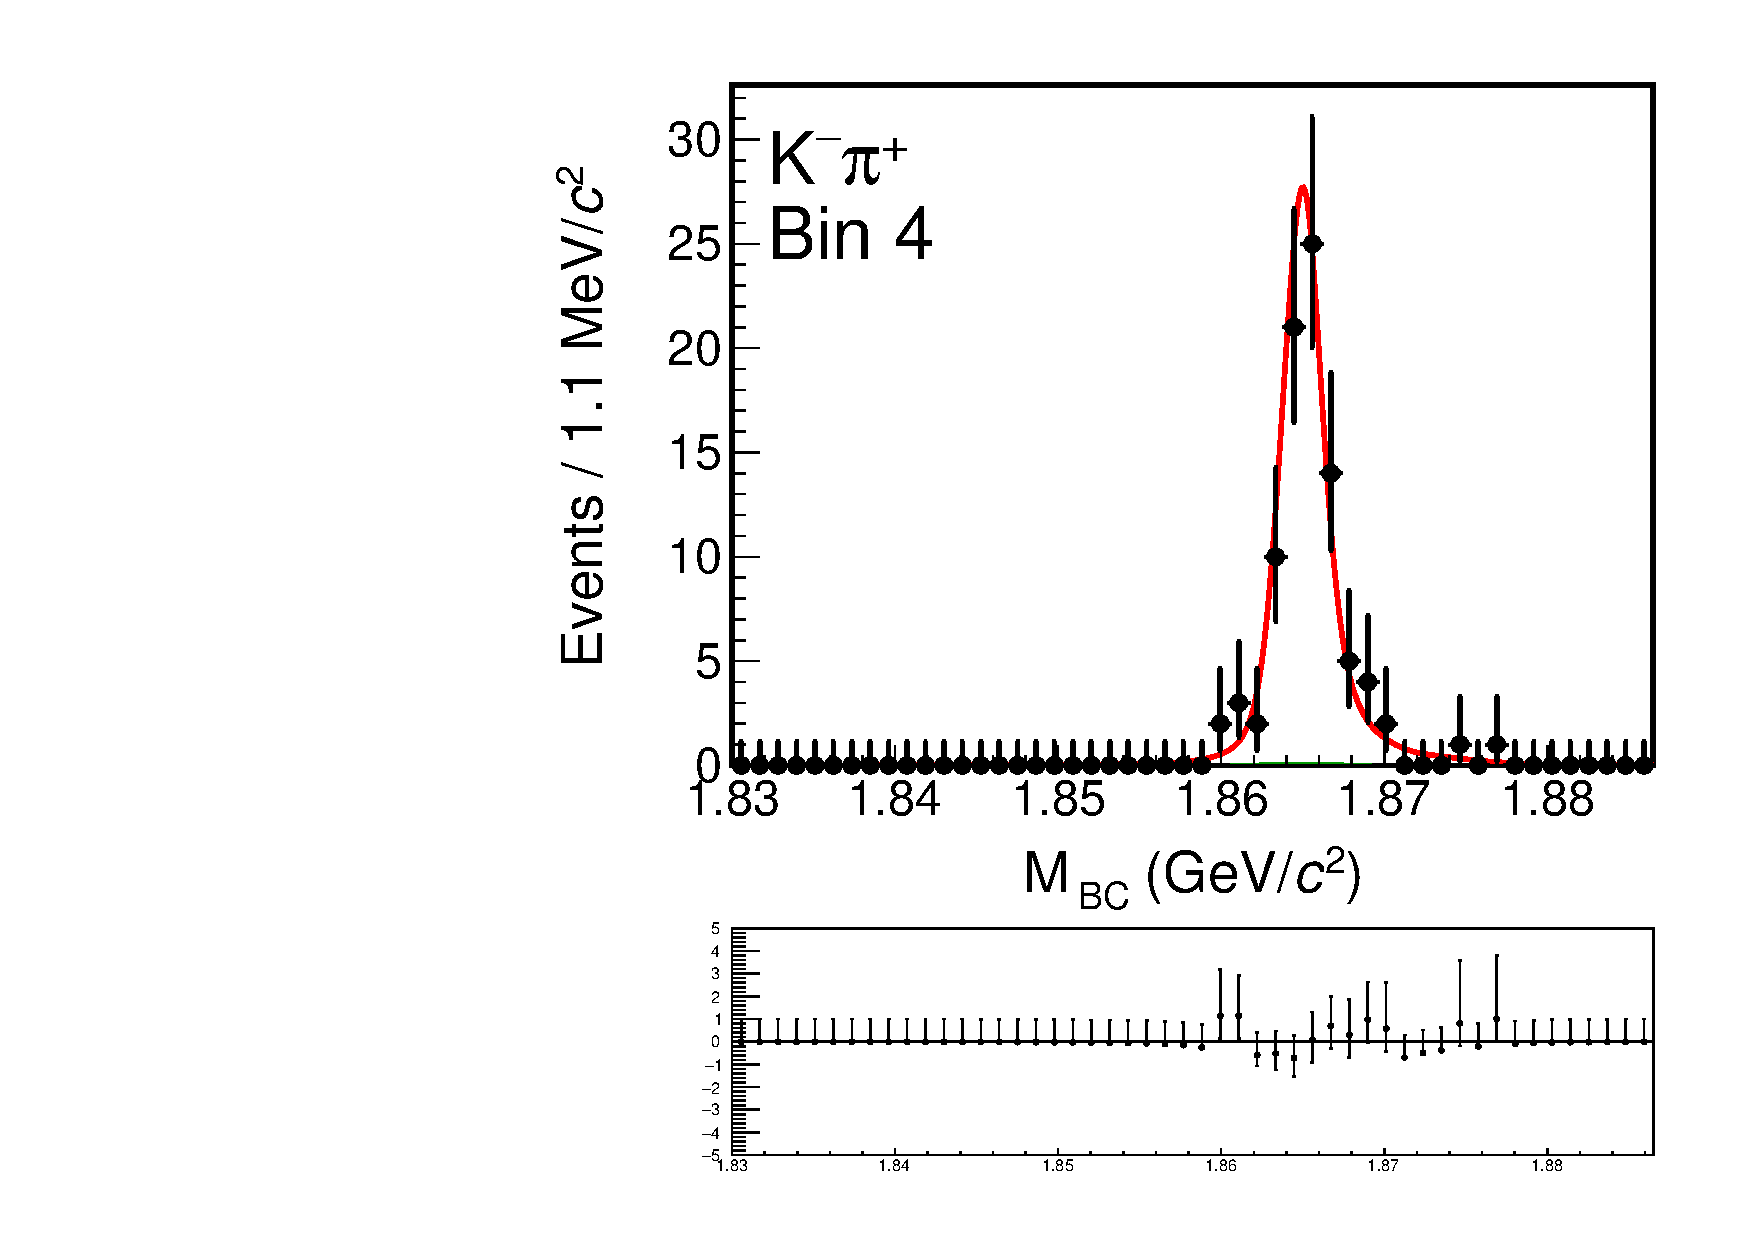
\includegraphics[width=0.75\textwidth,trim={0 5cm 0 0},clip=true]{Plots/DoubleTagYield_DoubleTag_Flavour_KKpipi_vs_Kpi_SignalBinP4_TagBin0.pdf}
      \caption{Bin $4$ yield: $88.6_{-9.0}^{+9.7}$}
    \end{subfigure}
  \end{figure}
\end{frame}

\begin{frame}{Double tag fit of $KK\pi\pi$ vs $KK$}
  \begin{figure}
    \centering
    \begin{subfigure}{0.5\textwidth}
      \centering
      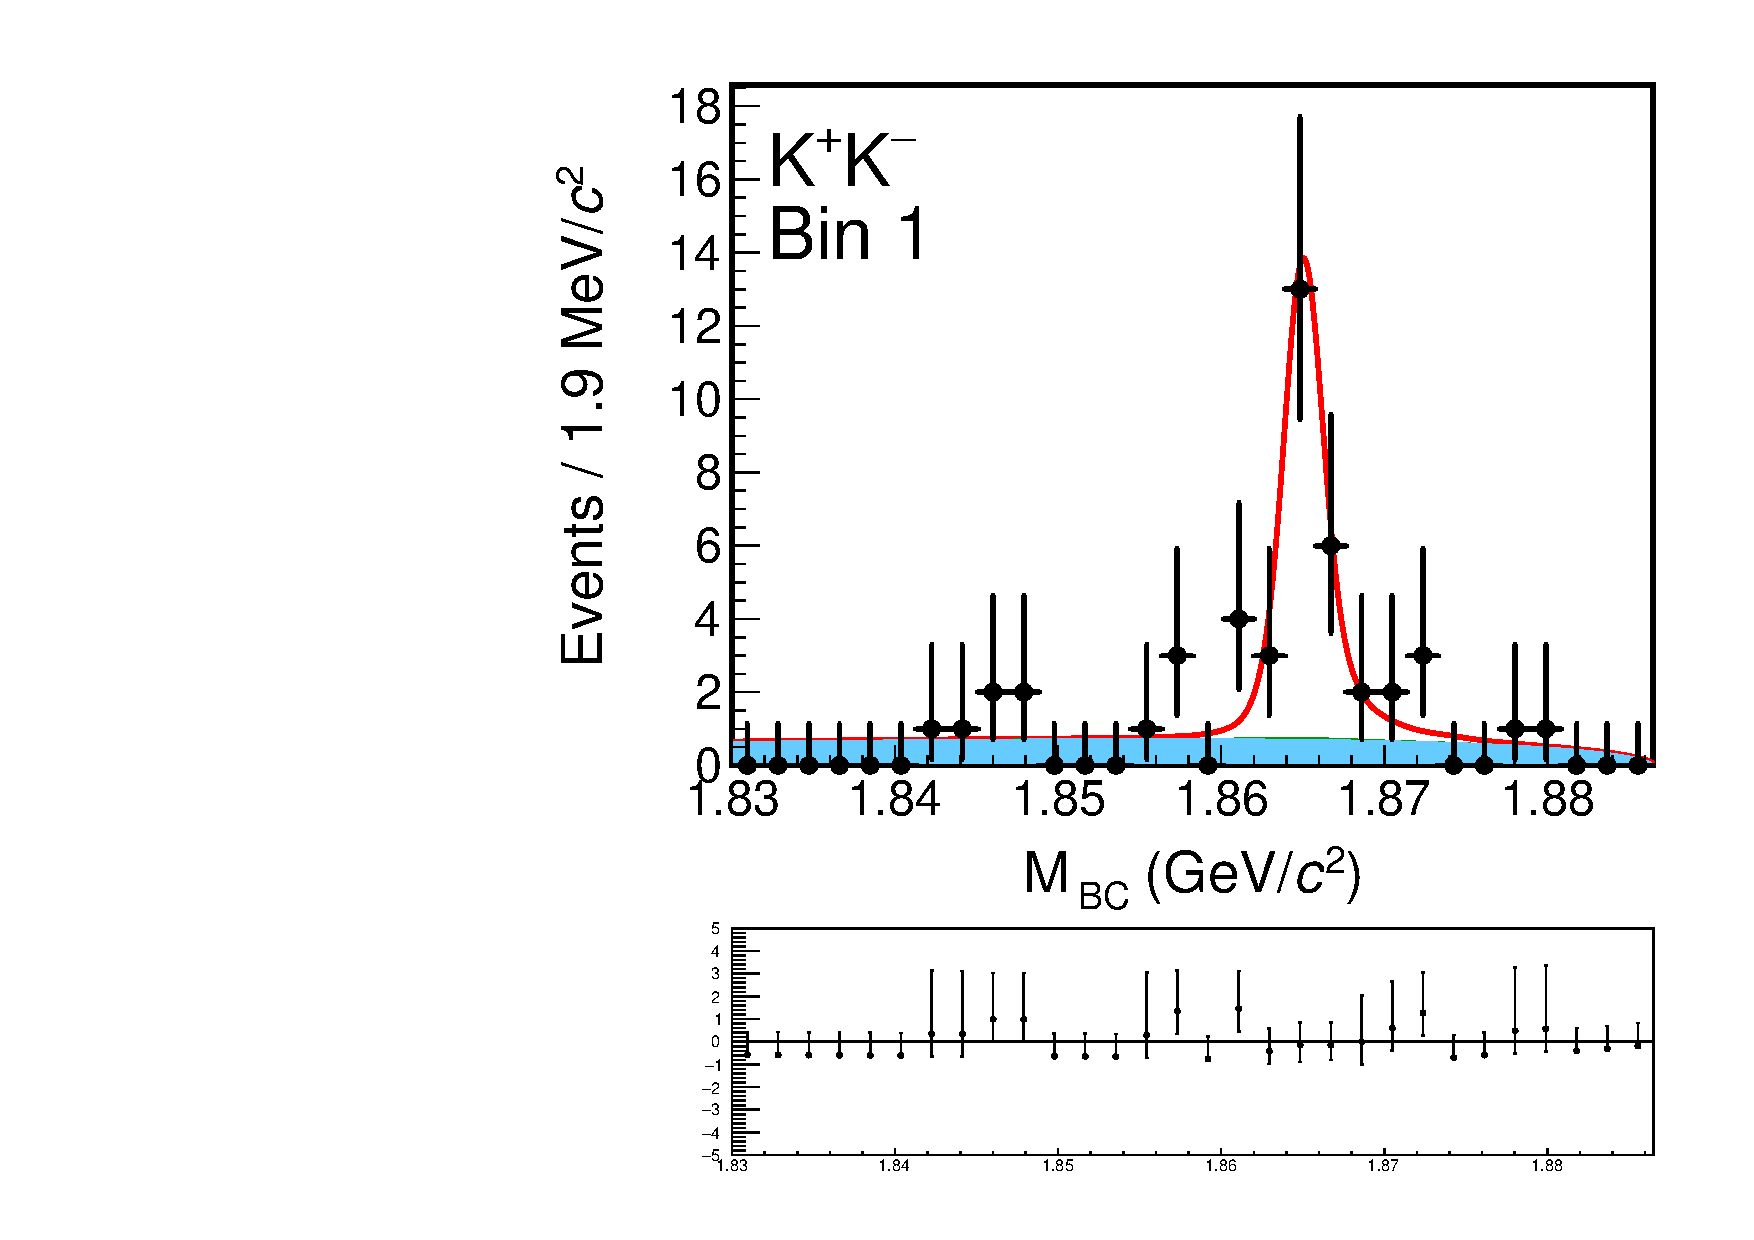
\includegraphics[width=0.75\textwidth,trim={0 5cm 0 0},clip=true]{Plots/DoubleTagYield_DoubleTag_CP_KKpipi_vs_KK_SignalBin1.pdf}
      \caption{Bin $1$ yield: $25.3_{-5.5}^{+6.2}$}
    \end{subfigure}%
    \begin{subfigure}{0.5\textwidth}
      \centering
      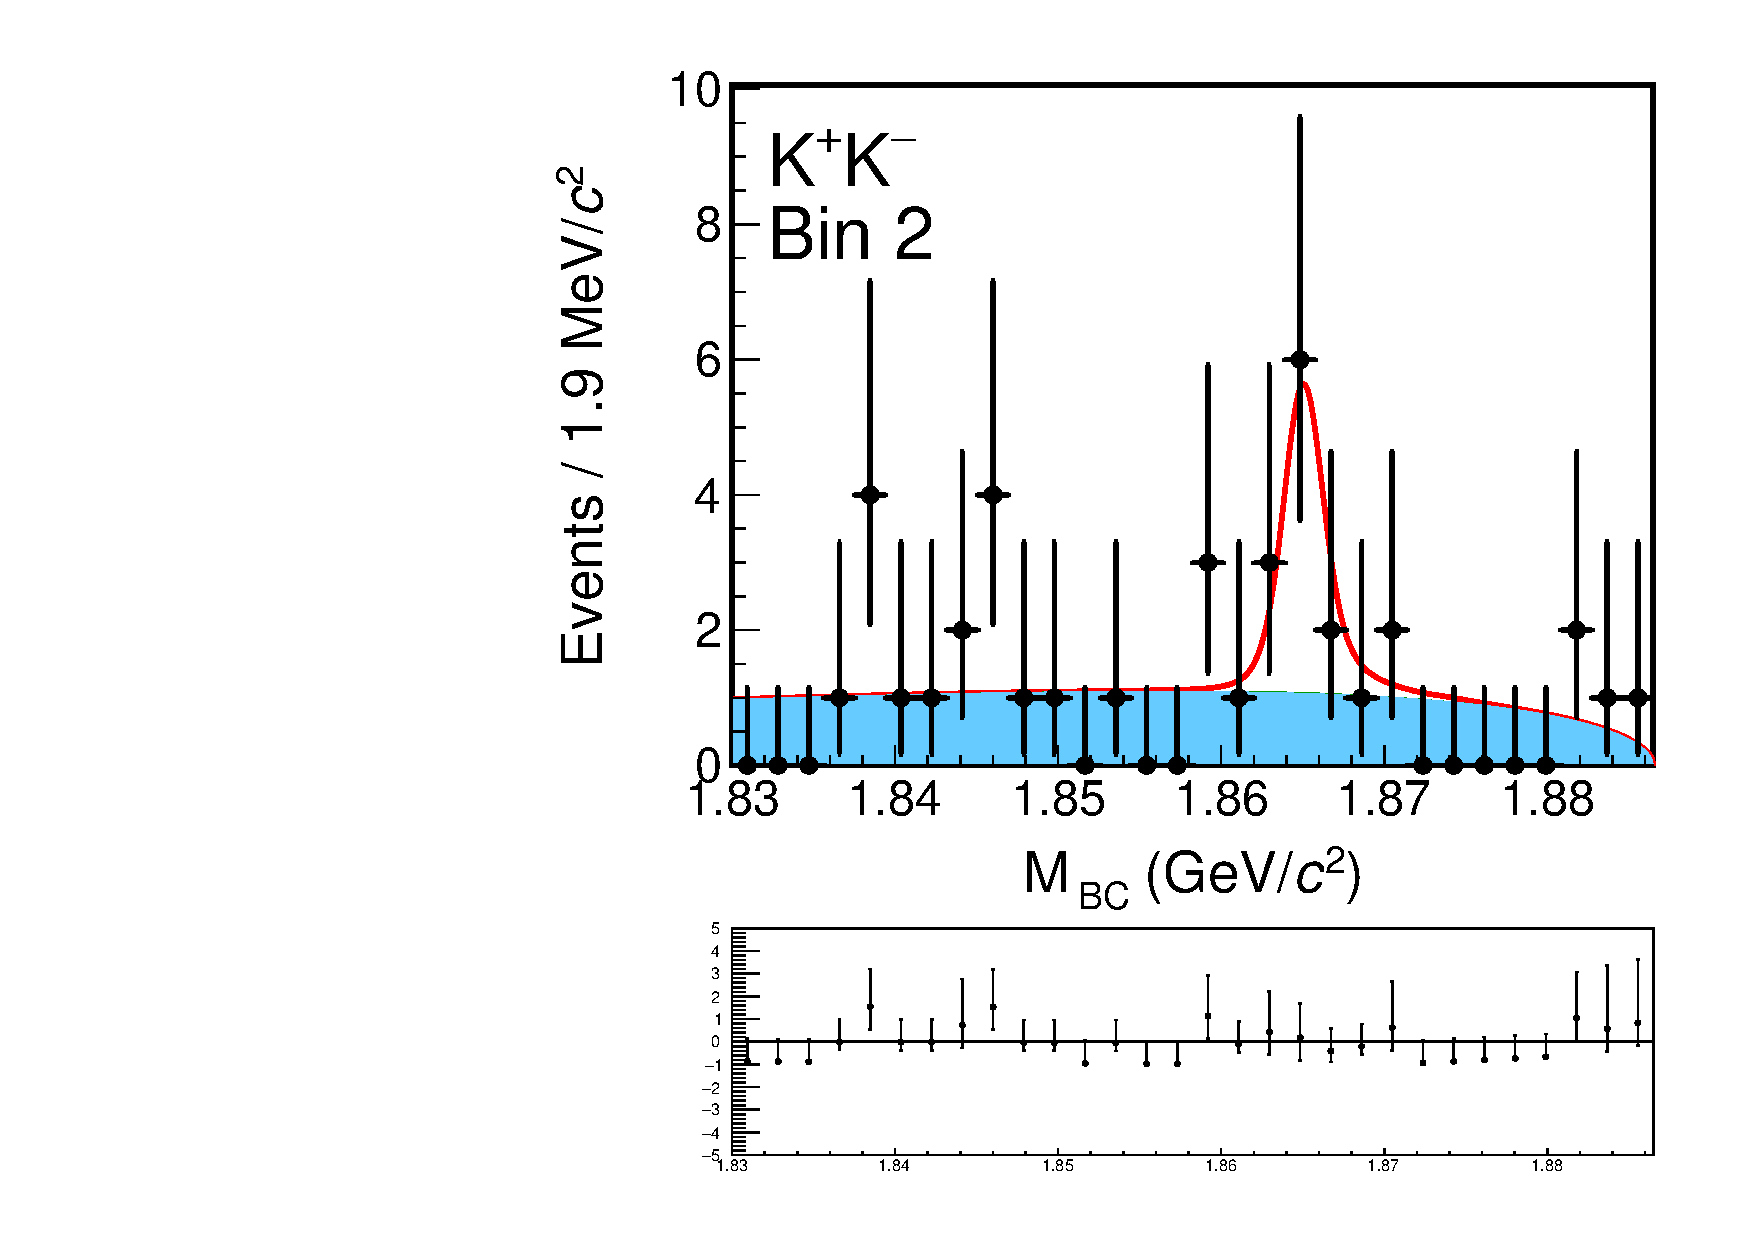
\includegraphics[width=0.75\textwidth,trim={0 5cm 0 0},clip=true]{Plots/DoubleTagYield_DoubleTag_CP_KKpipi_vs_KK_SignalBin2.pdf}
      \caption{Bin $2$ yield: $8.8_{-3.3}^{+4.0}$}
    \end{subfigure}
    \begin{subfigure}{0.5\textwidth}
      \centering
      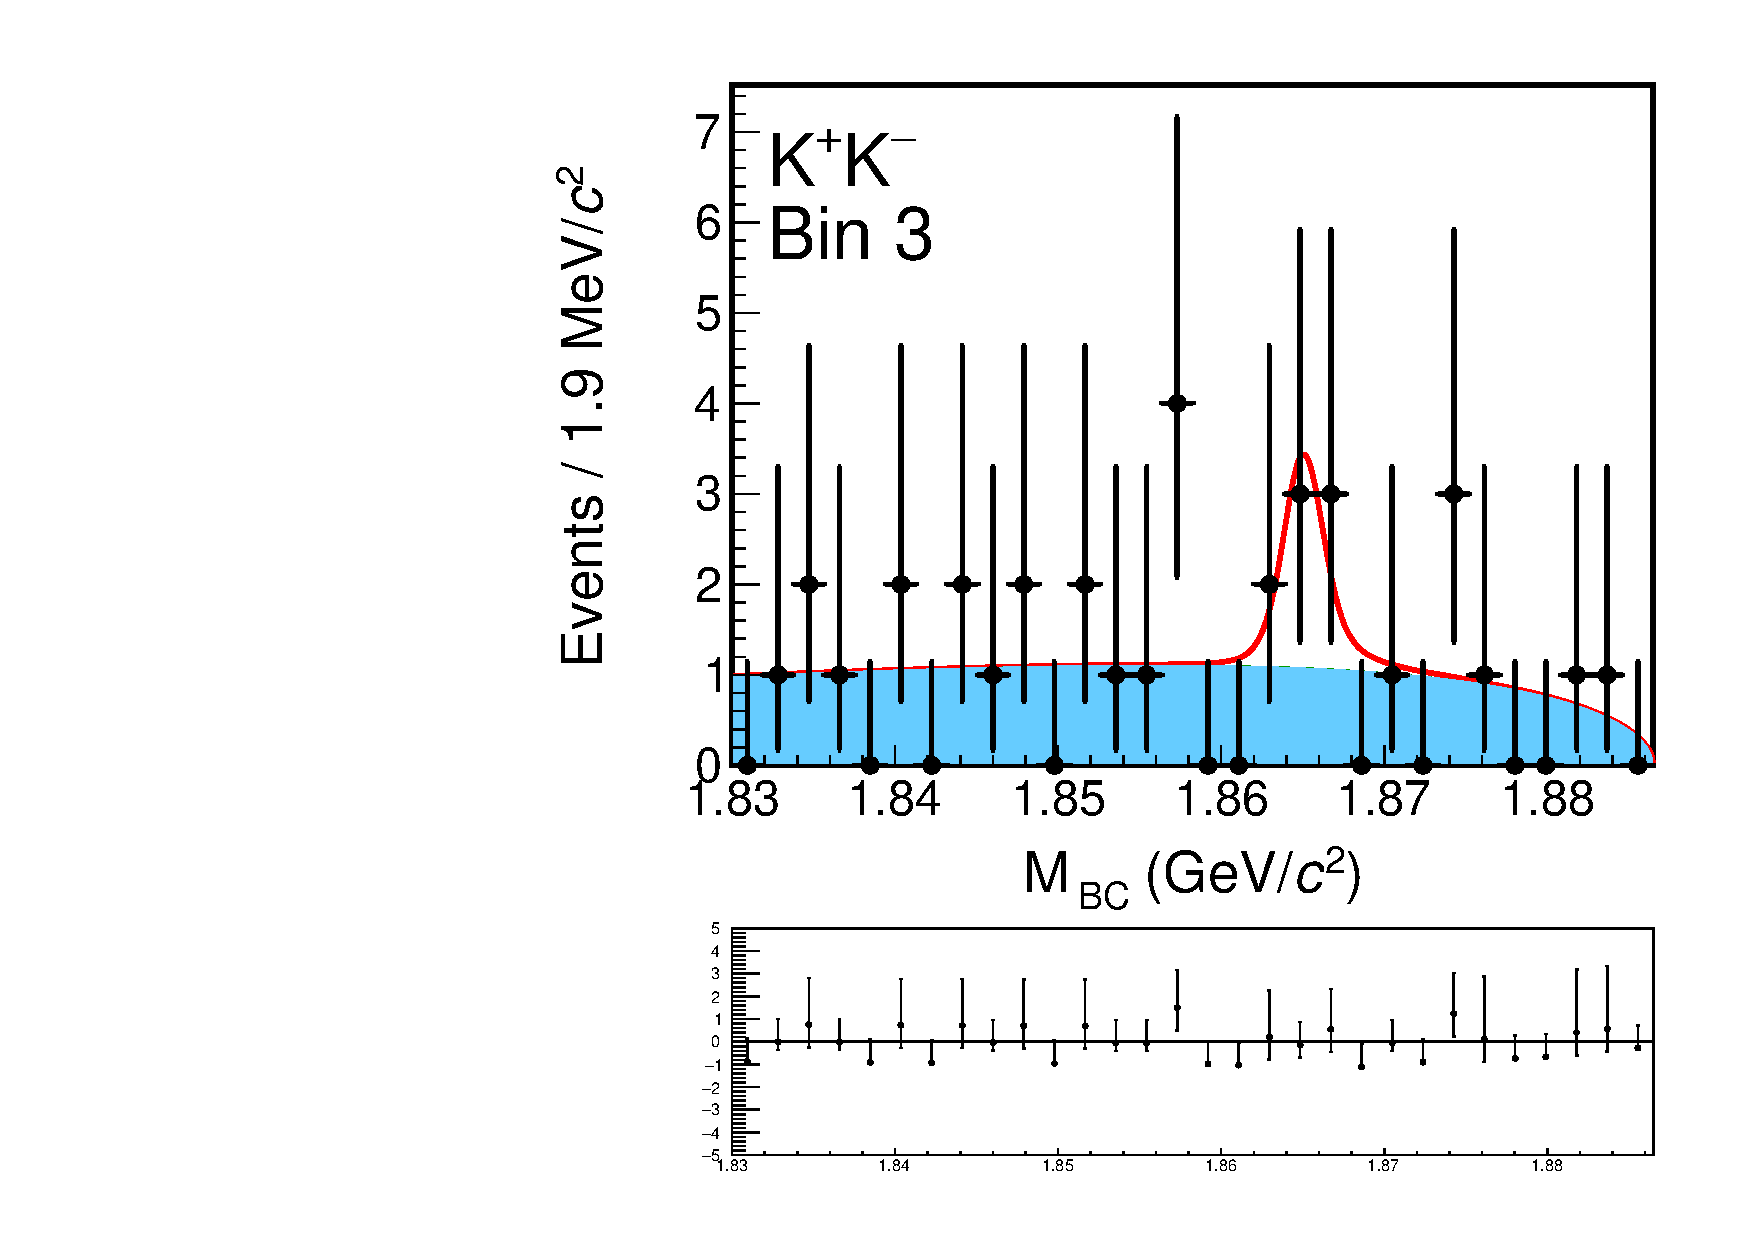
\includegraphics[width=0.75\textwidth,trim={0 5cm 0 0},clip=true]{Plots/DoubleTagYield_DoubleTag_CP_KKpipi_vs_KK_SignalBin3.pdf}
      \caption{Bin $3$ yield: $4.5_{-2.6}^{+3.3}$}
    \end{subfigure}%
    \begin{subfigure}{0.5\textwidth}
      \centering
      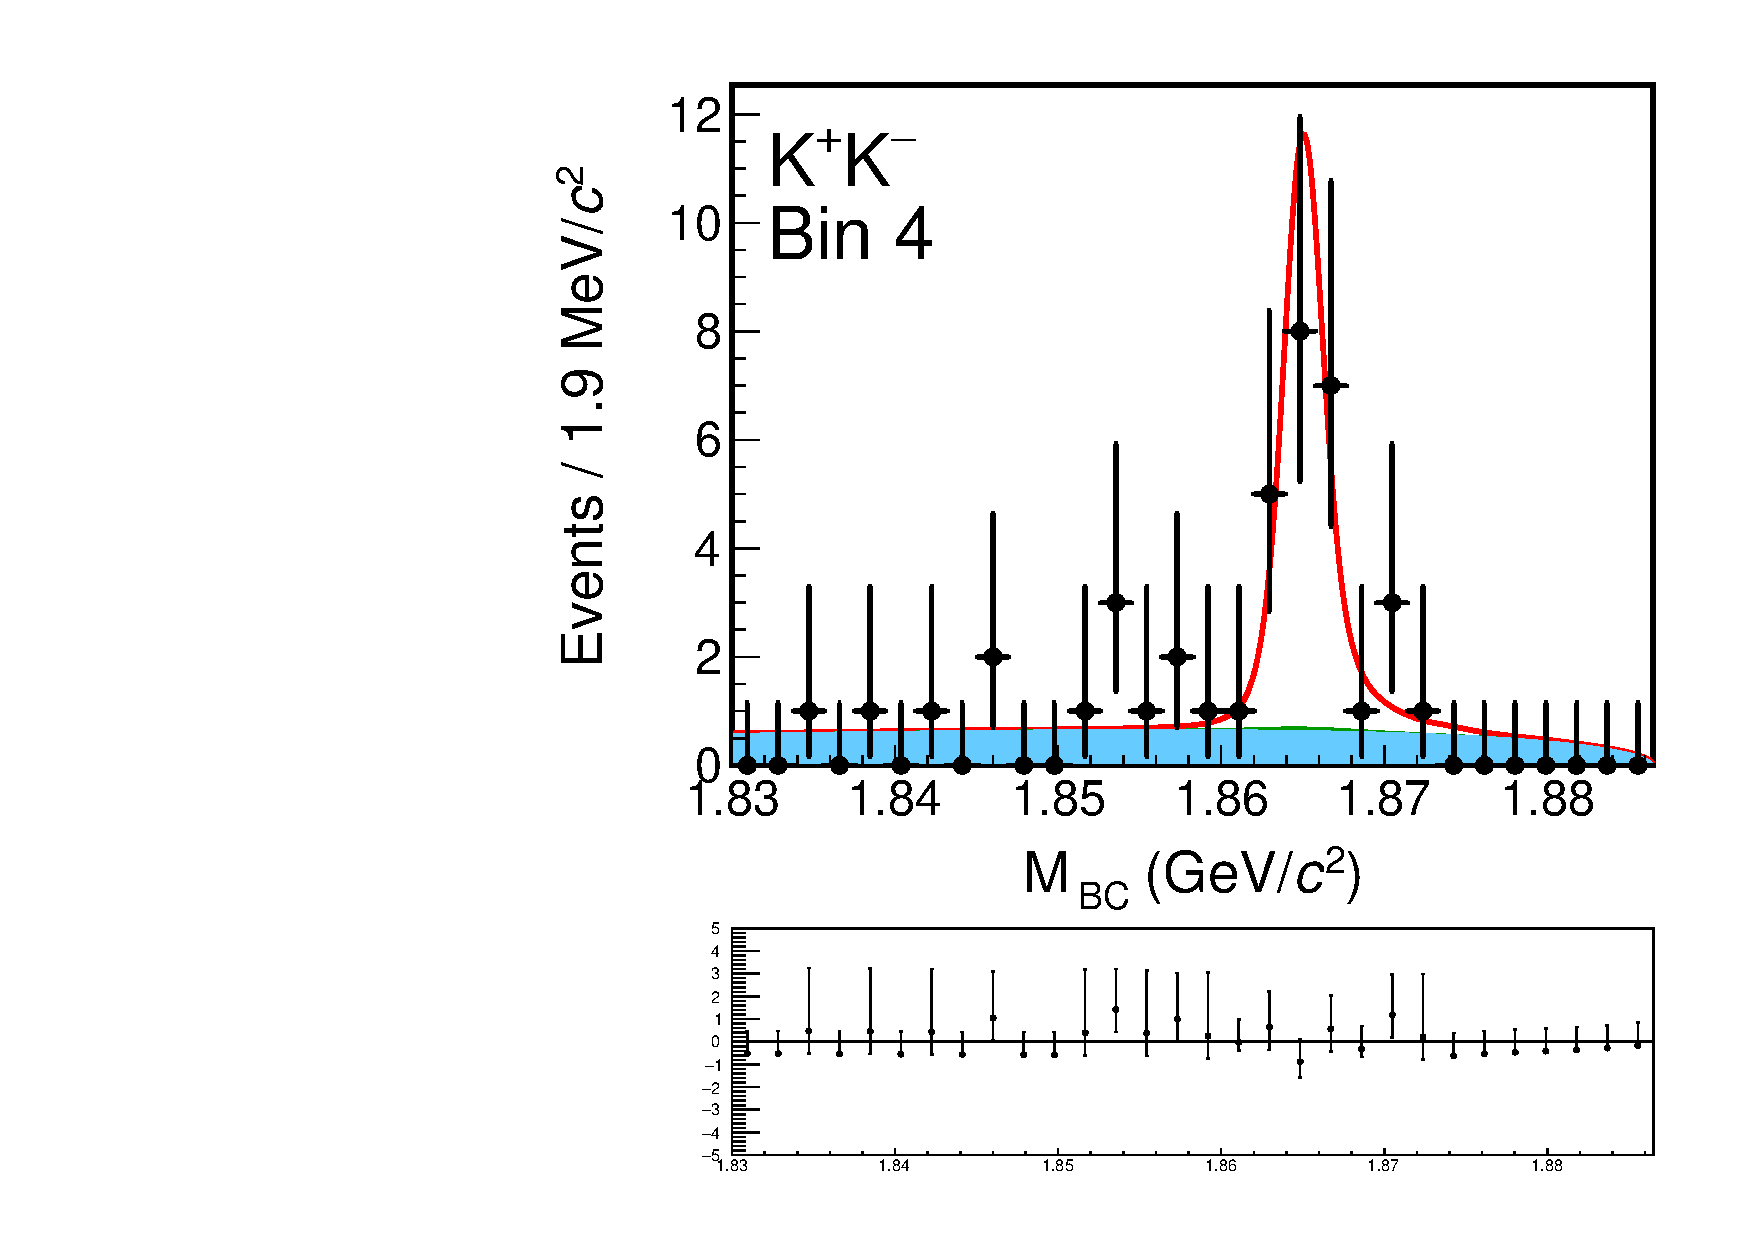
\includegraphics[width=0.75\textwidth,trim={0 5cm 0 0},clip=true]{Plots/DoubleTagYield_DoubleTag_CP_KKpipi_vs_KK_SignalBin4.pdf}
      \caption{Bin $4$ yield: $21.1_{-4.8}^{+5.5}$}
    \end{subfigure}
  \end{figure}
\end{frame}

\begin{frame}{Double tag fit of $KK\pi\pi$ vs $K_S\pi^0$}
  \begin{figure}
    \centering
    \begin{subfigure}{0.5\textwidth}
      \centering
      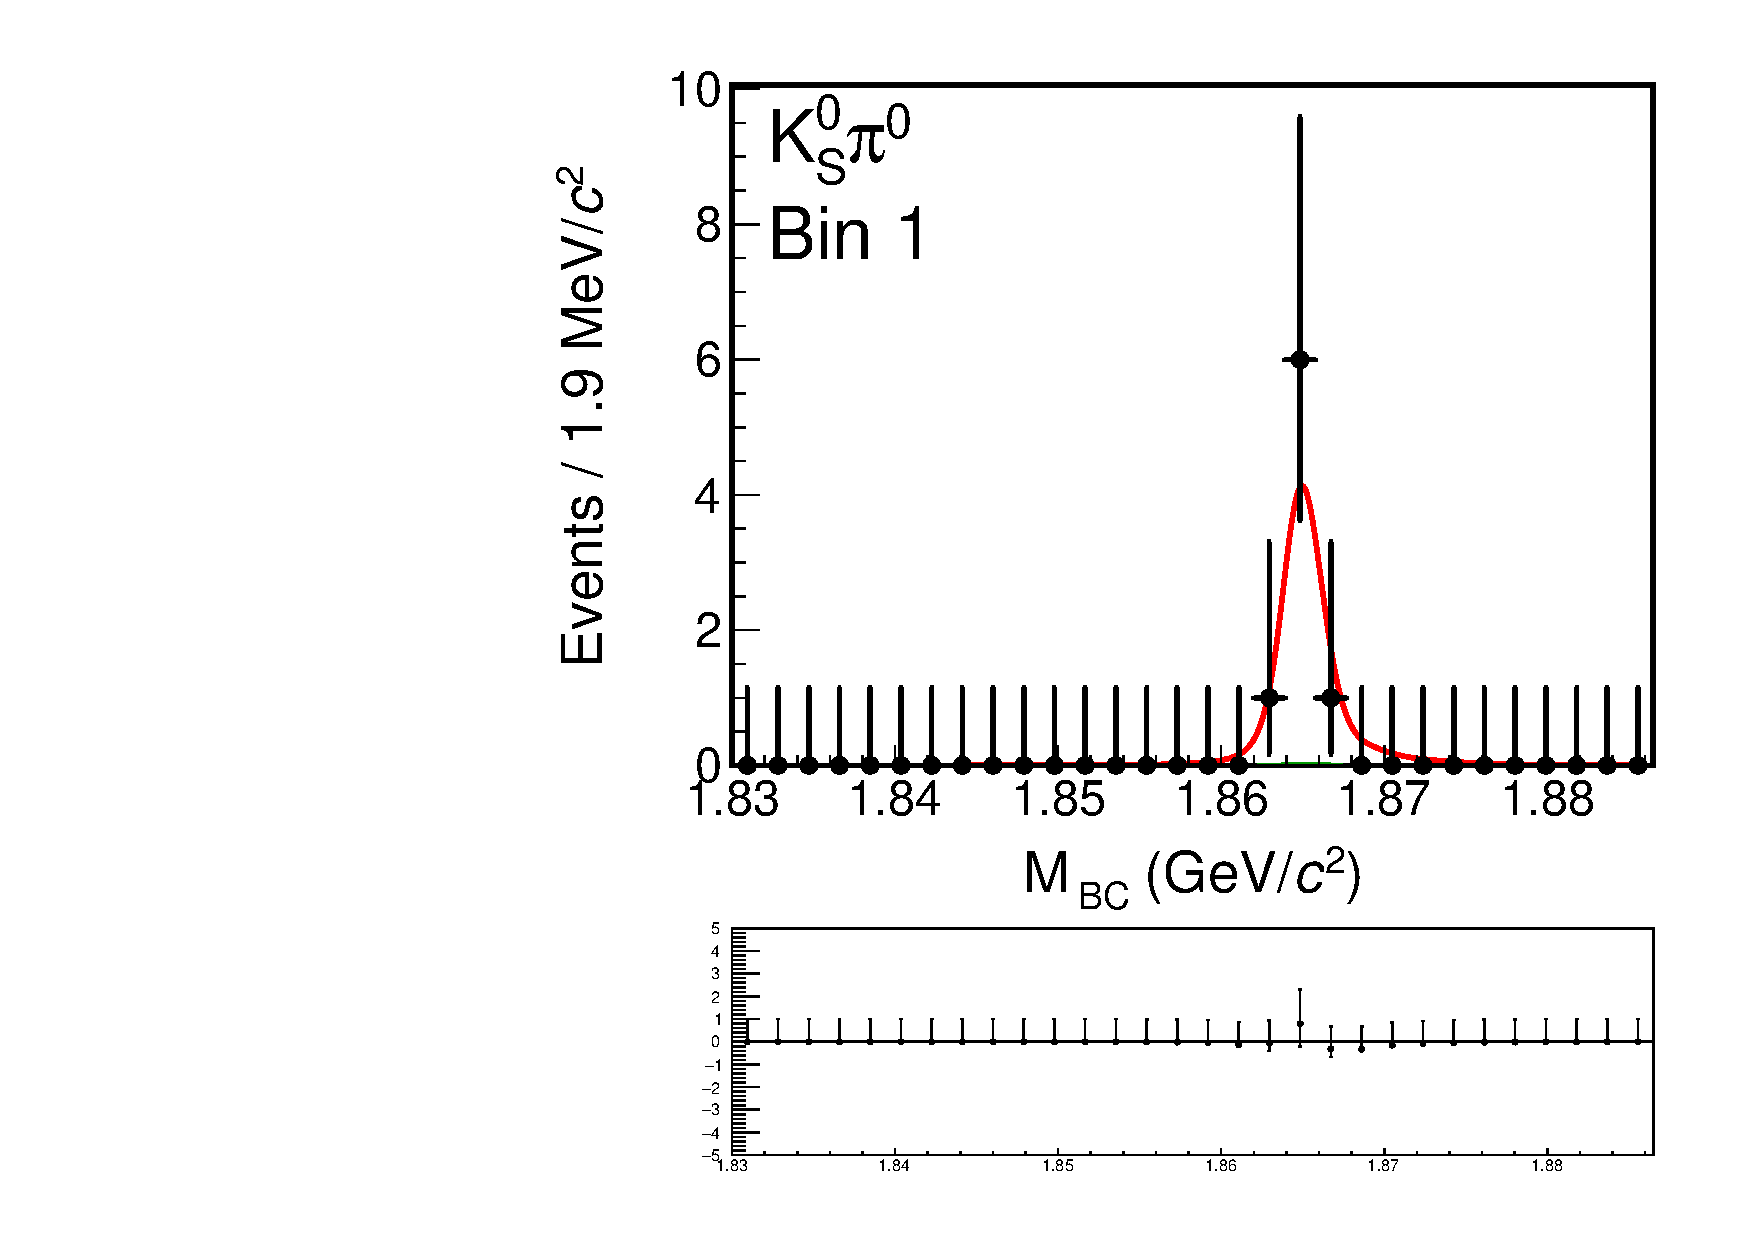
\includegraphics[width=0.75\textwidth,trim={0 5cm 0 0},clip=true]{Plots/DoubleTagYield_DoubleTag_CP_KKpipi_vs_KSpi0_SignalBin1.pdf}
      \caption{Bin $1$ yield: $7.9_{-2.5}^{+3.1}$}
    \end{subfigure}%
    \begin{subfigure}{0.5\textwidth}
      \centering
      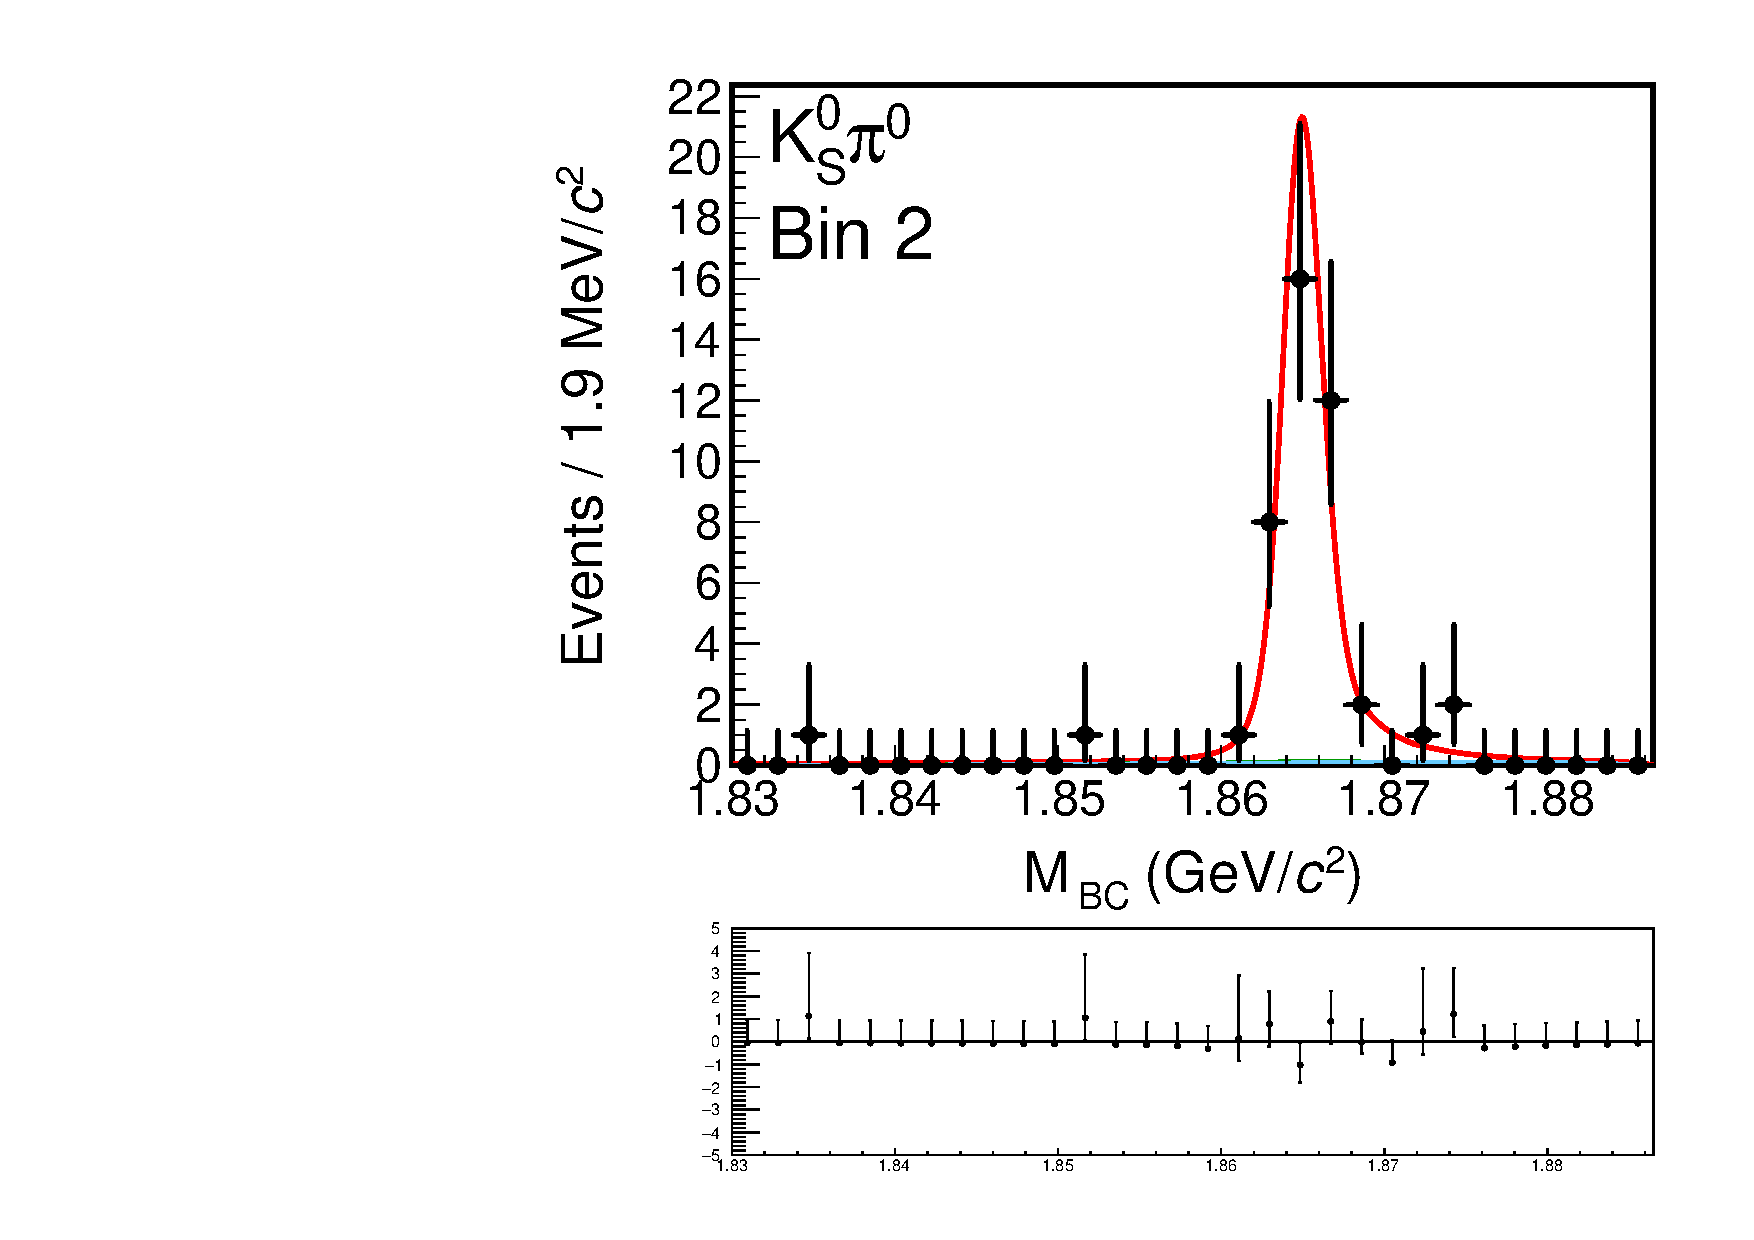
\includegraphics[width=0.75\textwidth,trim={0 5cm 0 0},clip=true]{Plots/DoubleTagYield_DoubleTag_CP_KKpipi_vs_KSpi0_SignalBin2.pdf}
      \caption{Bin $2$ yield: $40.4_{-6.3}^{+6.8}$}
    \end{subfigure}
    \begin{subfigure}{0.5\textwidth}
      \centering
      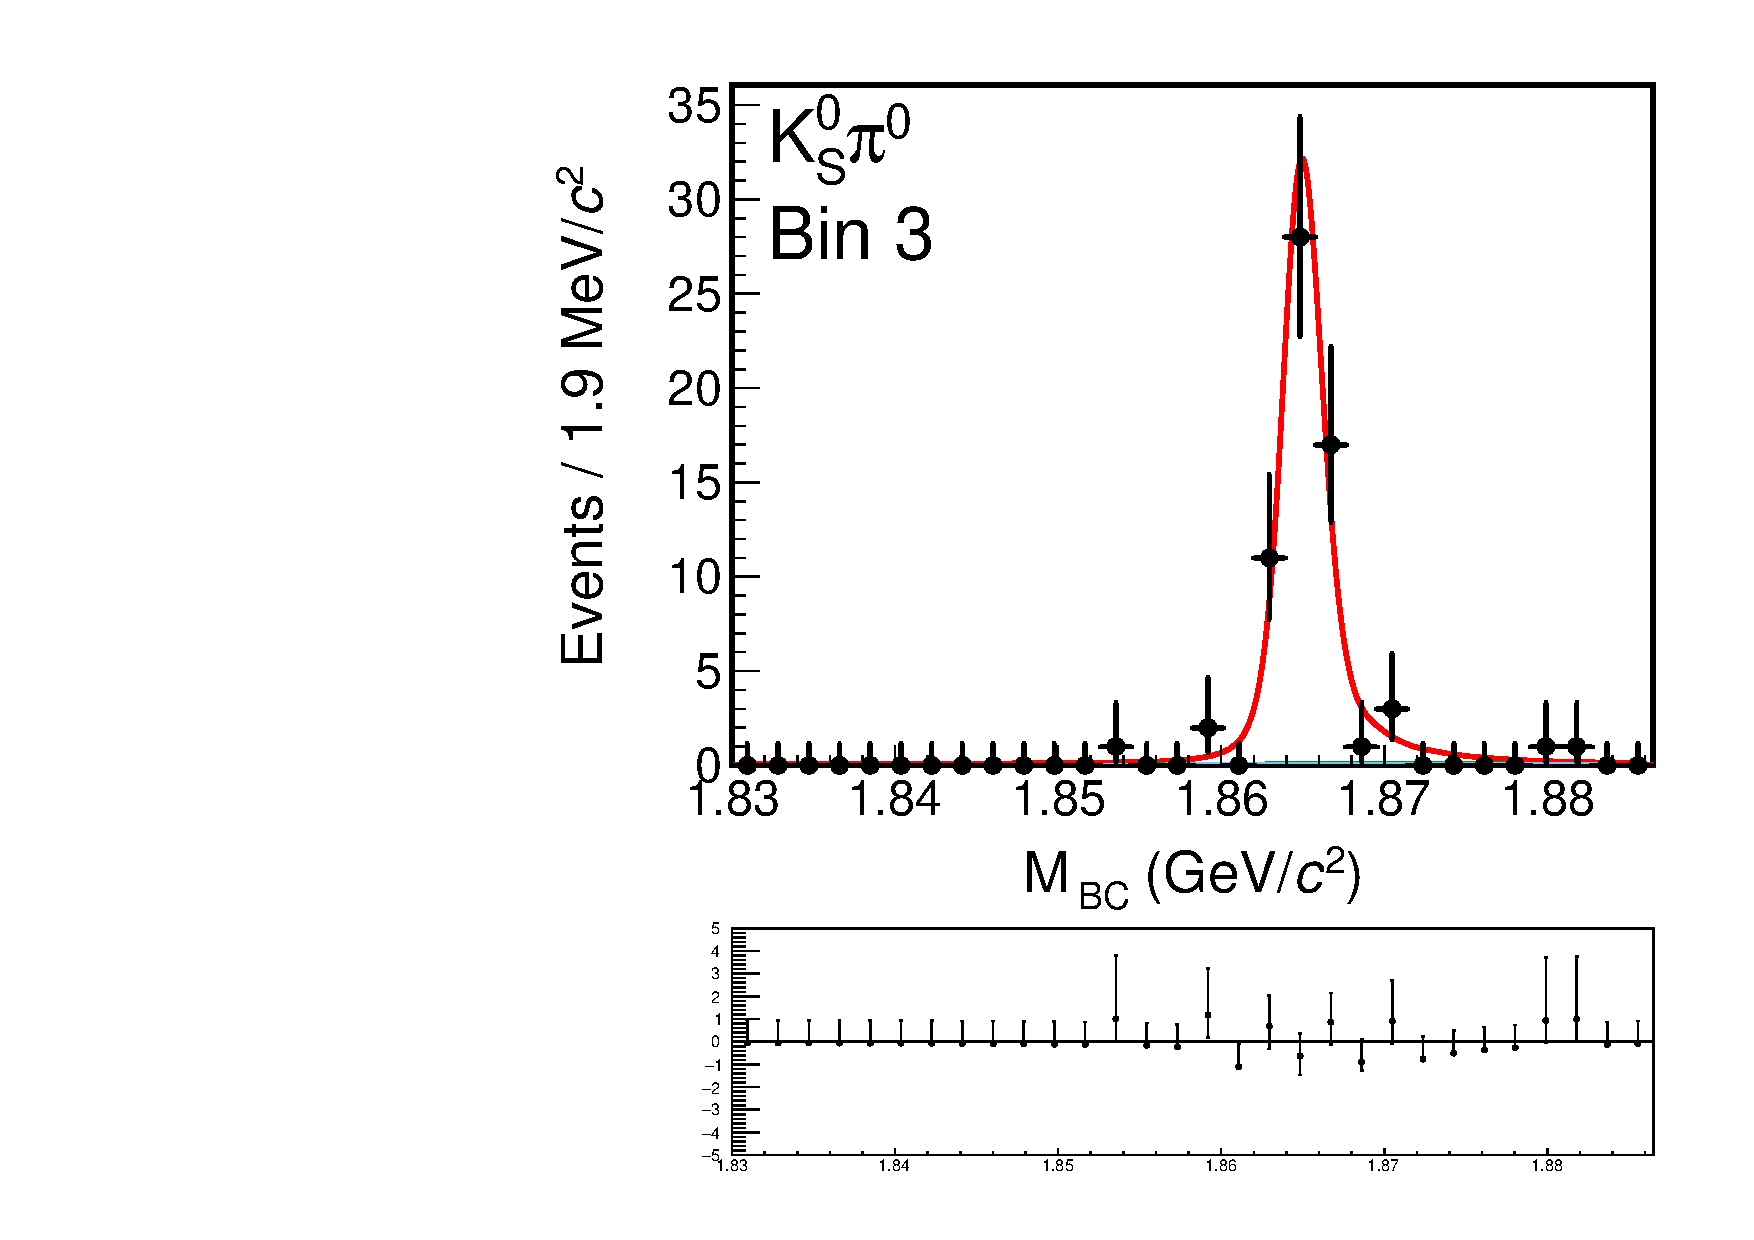
\includegraphics[width=0.75\textwidth,trim={0 5cm 0 0},clip=true]{Plots/DoubleTagYield_DoubleTag_CP_KKpipi_vs_KSpi0_SignalBin3.pdf}
      \caption{Bin $3$ yield: $61.1_{-7.8}^{+8.3}$}
    \end{subfigure}%
    \begin{subfigure}{0.5\textwidth}
      \centering
      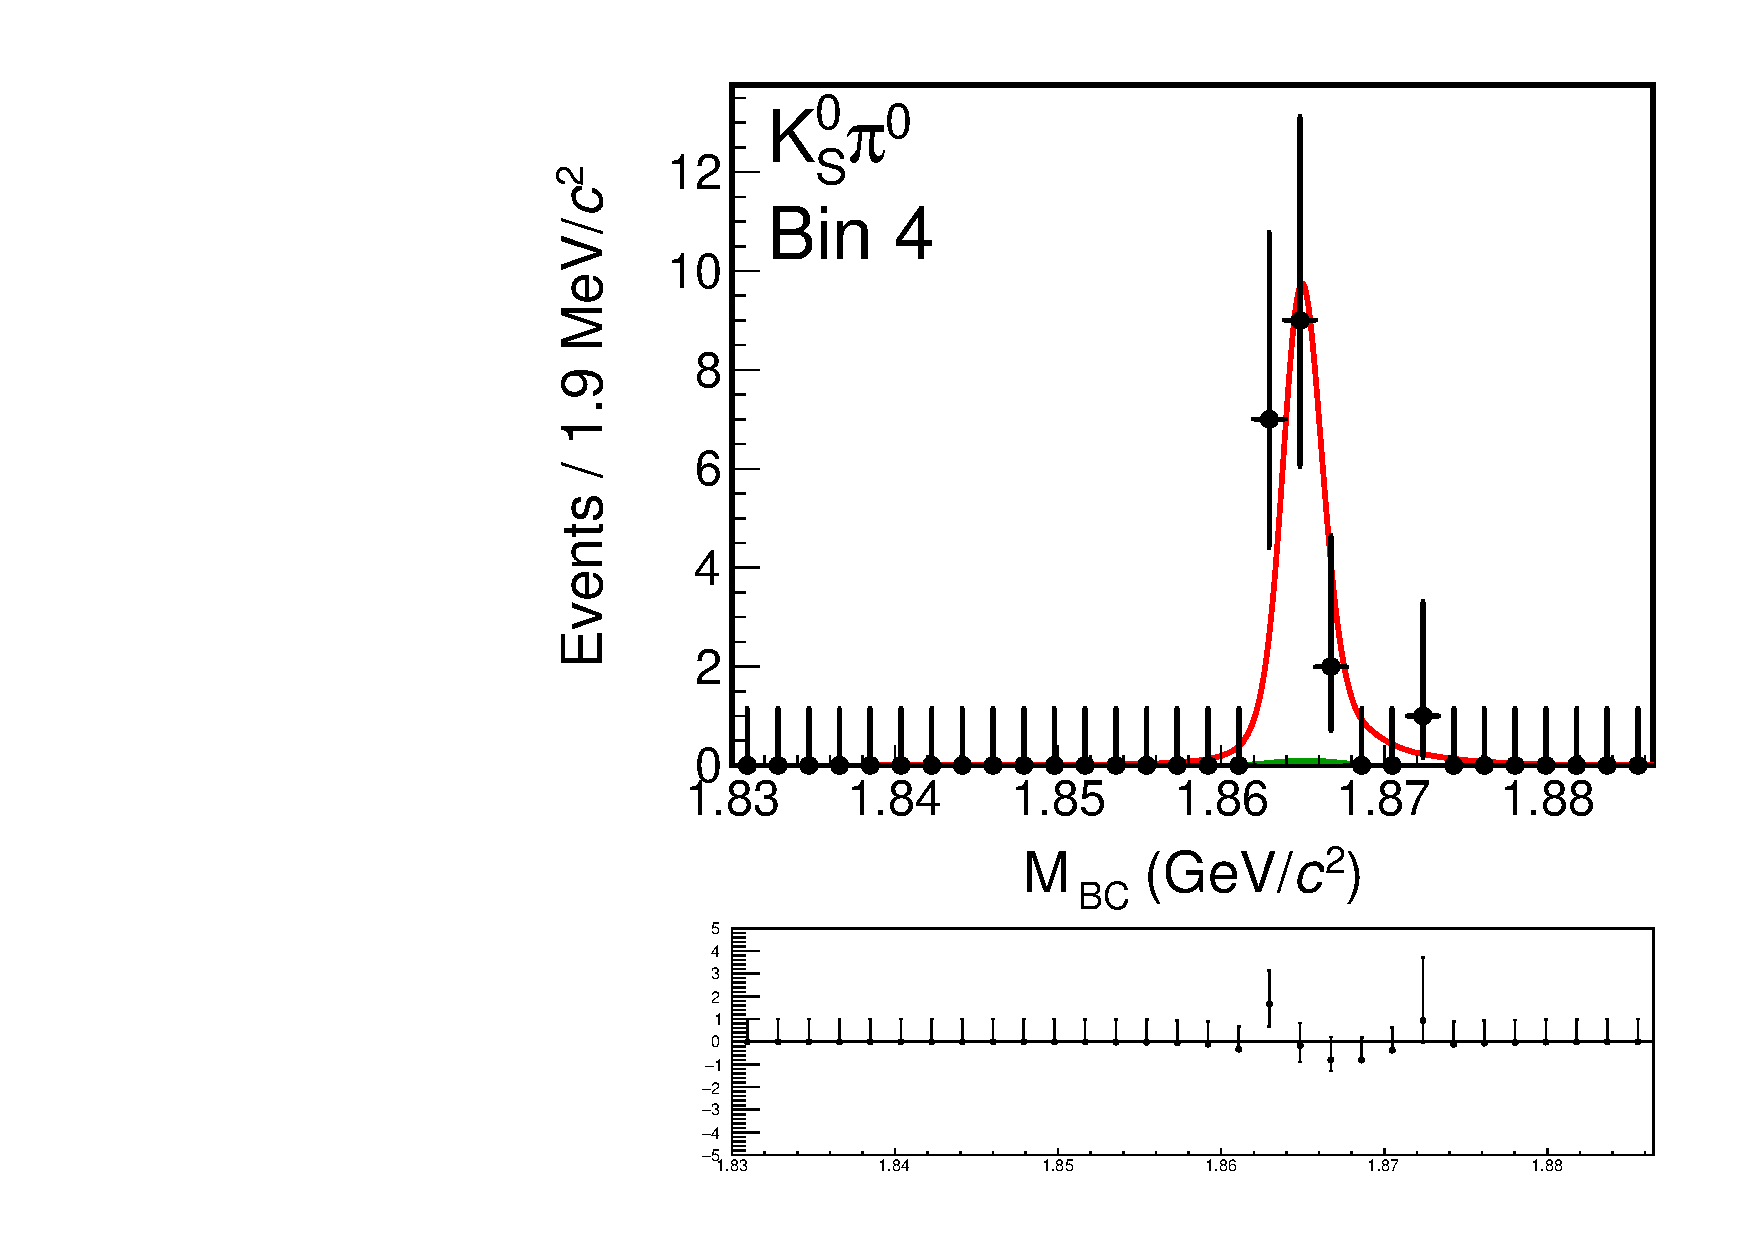
\includegraphics[width=0.75\textwidth,trim={0 5cm 0 0},clip=true]{Plots/DoubleTagYield_DoubleTag_CP_KKpipi_vs_KSpi0_SignalBin4.pdf}
      \caption{Bin $4$ yield: $18.3_{-3.9}^{+4.5}$}
    \end{subfigure}
  \end{figure}
\end{frame}

\begin{frame}{Double tag fit of $KK\pi\pi$ vs $K_S\pi^+\pi^-$}
  \begin{figure}
    \centering
    \begin{subfigure}{0.5\textwidth}
      \centering
      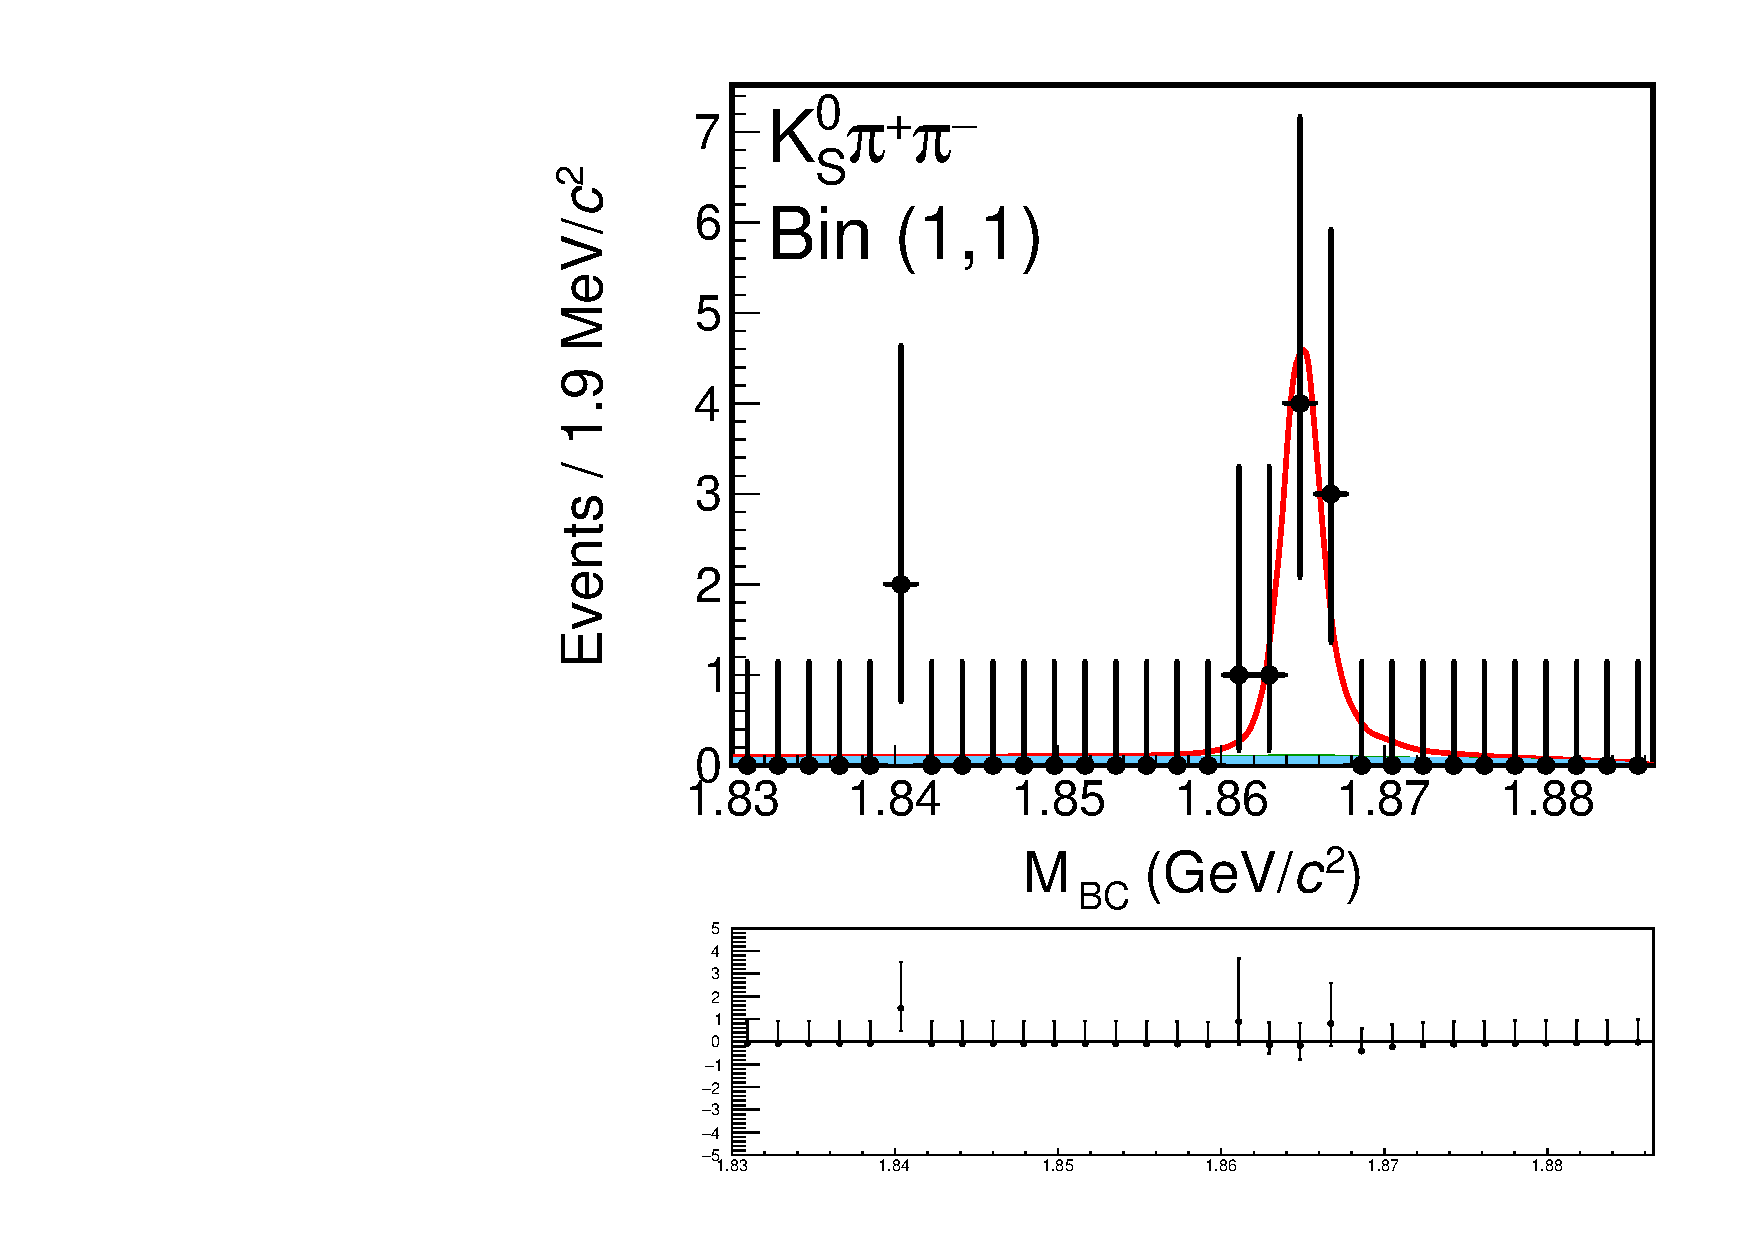
\includegraphics[width=0.75\textwidth,trim={0 5cm 0 0},clip=true]{Plots/DoubleTagYield_DoubleTag_SCMB_KKpipi_vs_KSpipi_SignalBinP1_TagBin1.pdf}
      \caption{Bin $(1, 1)$ yield: $8.2_{-2.7}^{+3.3}$}
    \end{subfigure}%
    \begin{subfigure}{0.5\textwidth}
      \centering
      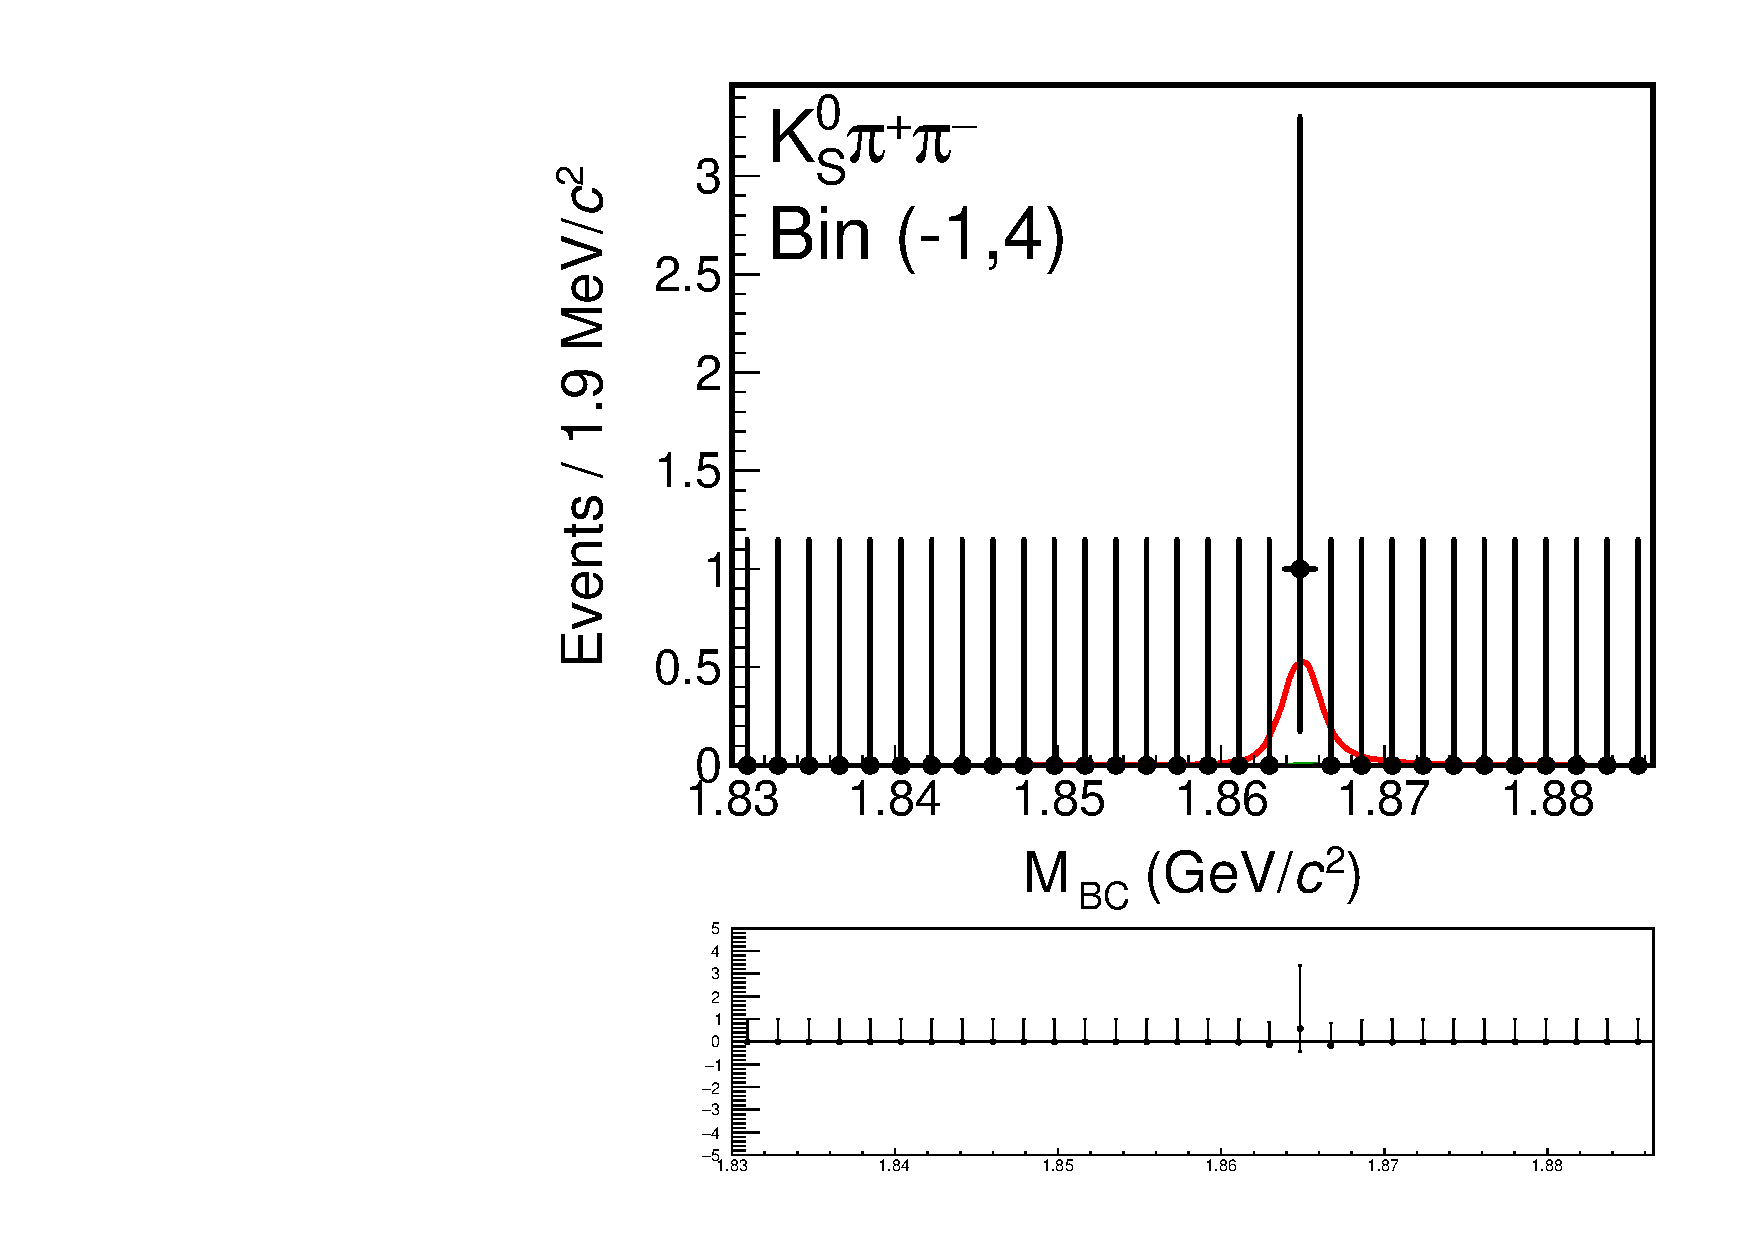
\includegraphics[width=0.75\textwidth,trim={0 5cm 0 0},clip=true]{Plots/DoubleTagYield_DoubleTag_SCMB_KKpipi_vs_KSpipi_SignalBinM1_TagBin4.pdf}
      \caption{Bin $(-1, 4)$ yield: $0.9_{-0.7}^{+1.3}$}
    \end{subfigure}
  \end{figure}
\end{frame}

\begin{frame}{Toy studies}
  \begin{figure}
    \centering
    \begin{subfigure}{0.5\textwidth}
      \centering
      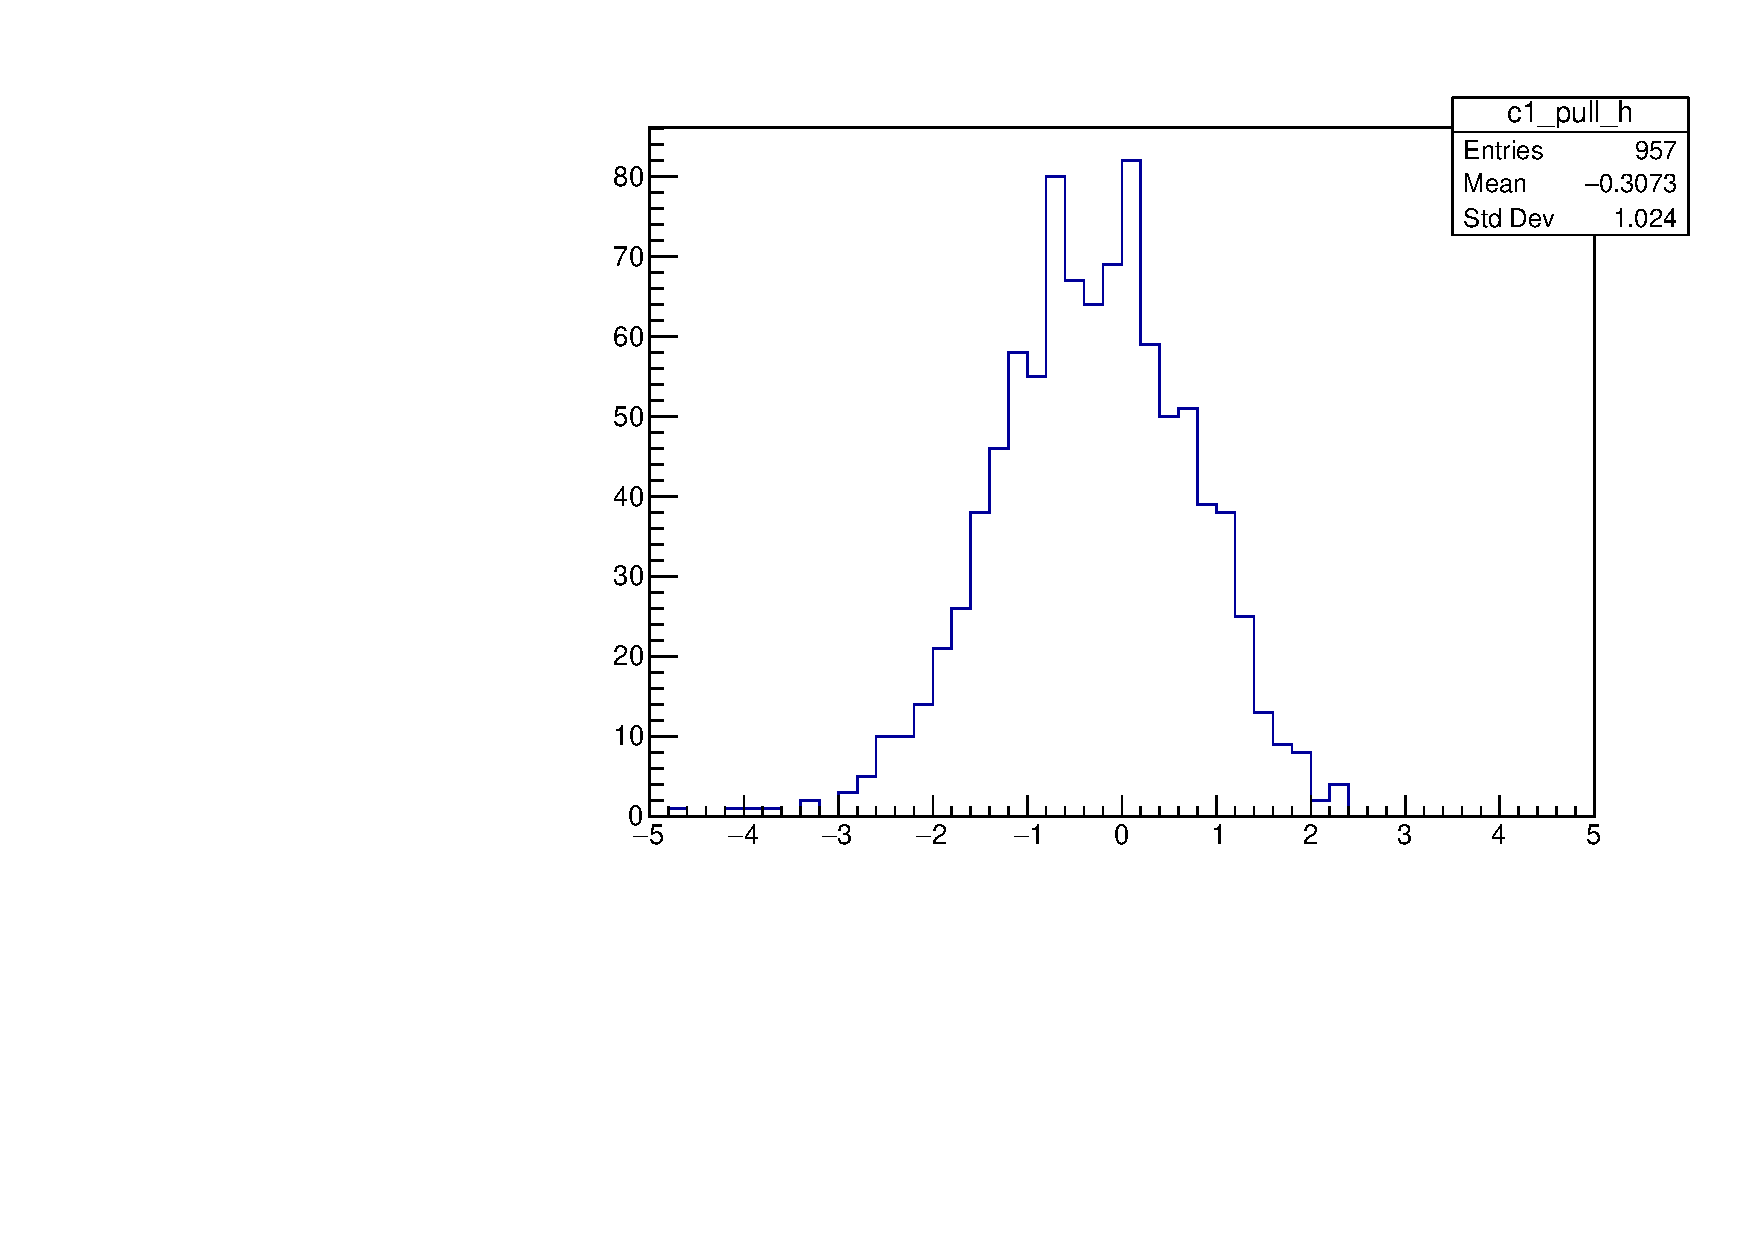
\includegraphics[width=0.75\textwidth,trim={0 0 0 0},clip=true]{Plots/c1_ToyFits_pull.pdf}
      \caption{$c_1$ pulls}
    \end{subfigure}%
    \begin{subfigure}{0.5\textwidth}
      \centering
      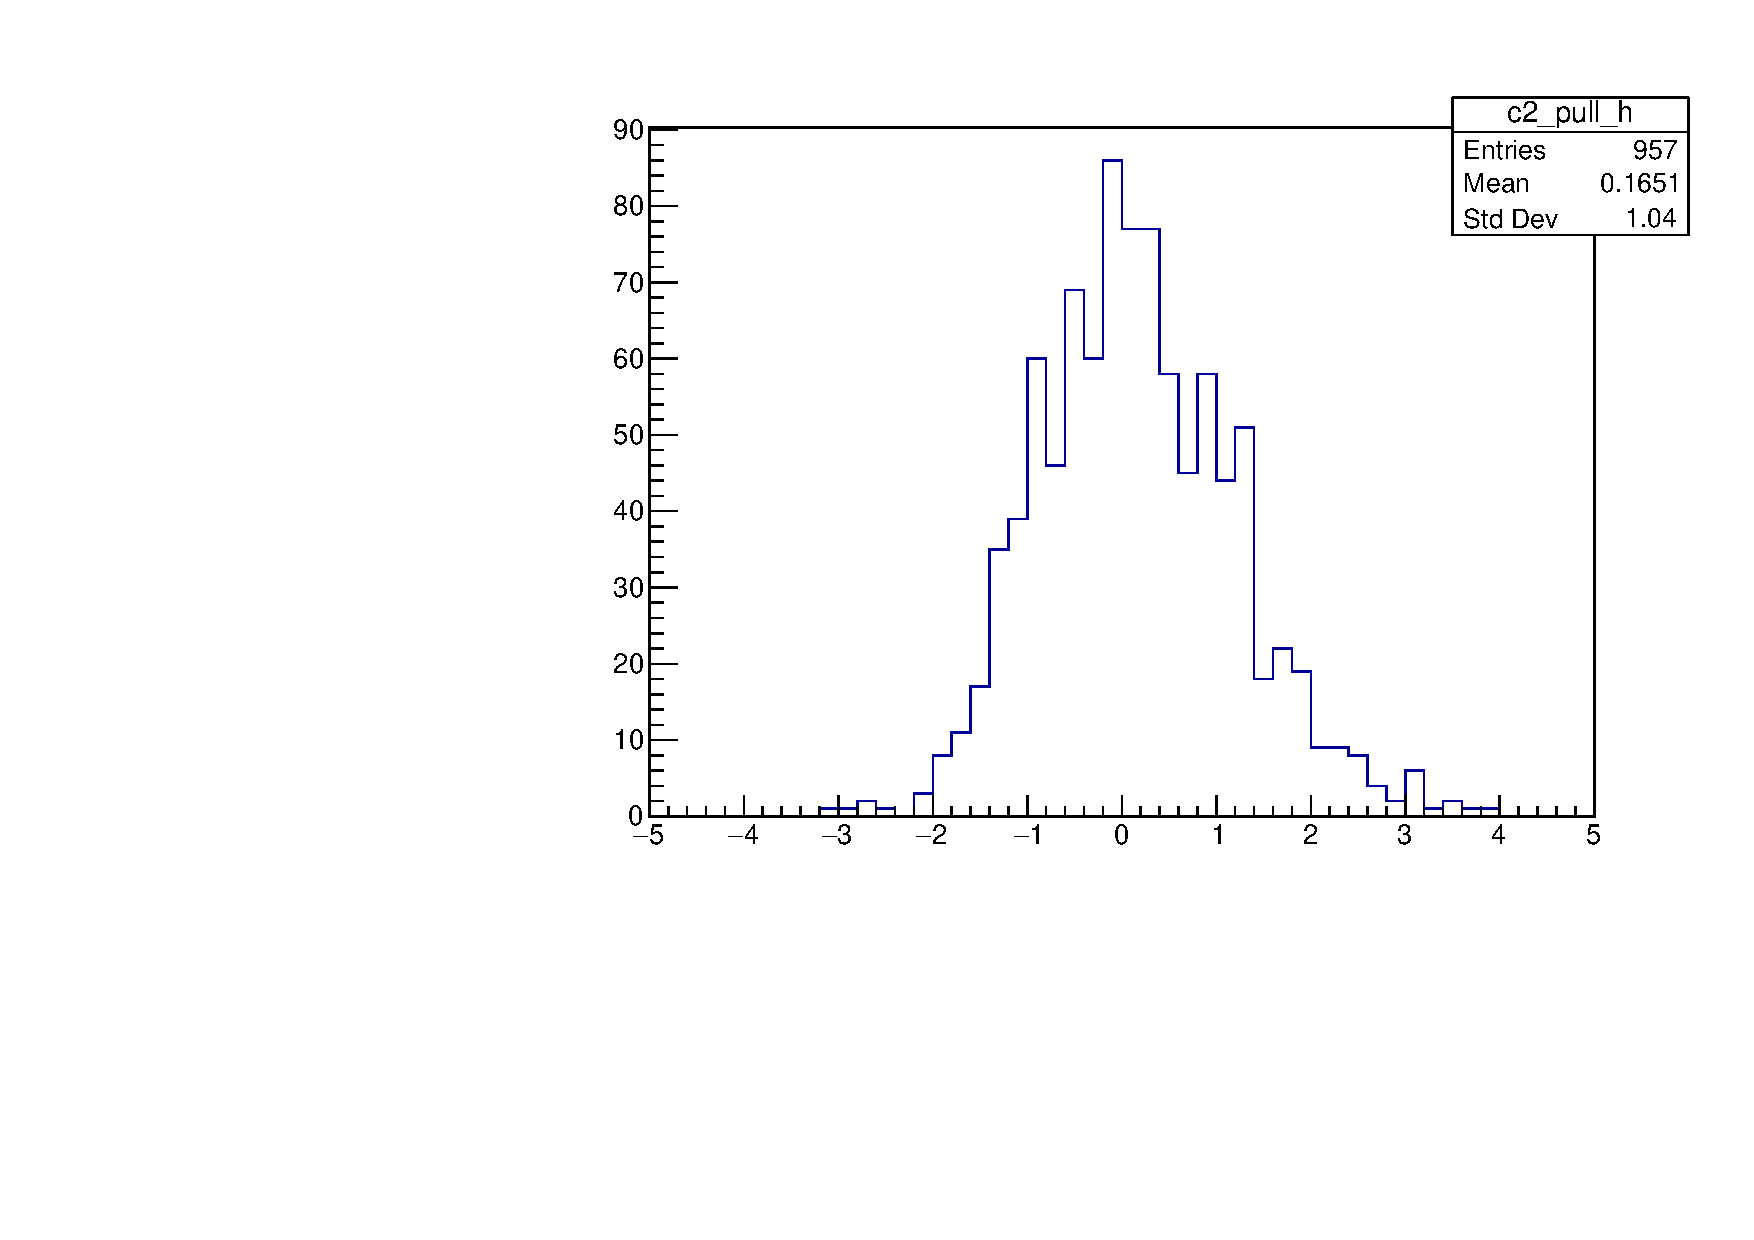
\includegraphics[width=0.75\textwidth,trim={0 0 0 0},clip=true]{Plots/c2_ToyFits_pull.pdf}
      \caption{$c_2$ pulls}
    \end{subfigure}
    \begin{subfigure}{0.5\textwidth}
      \centering
      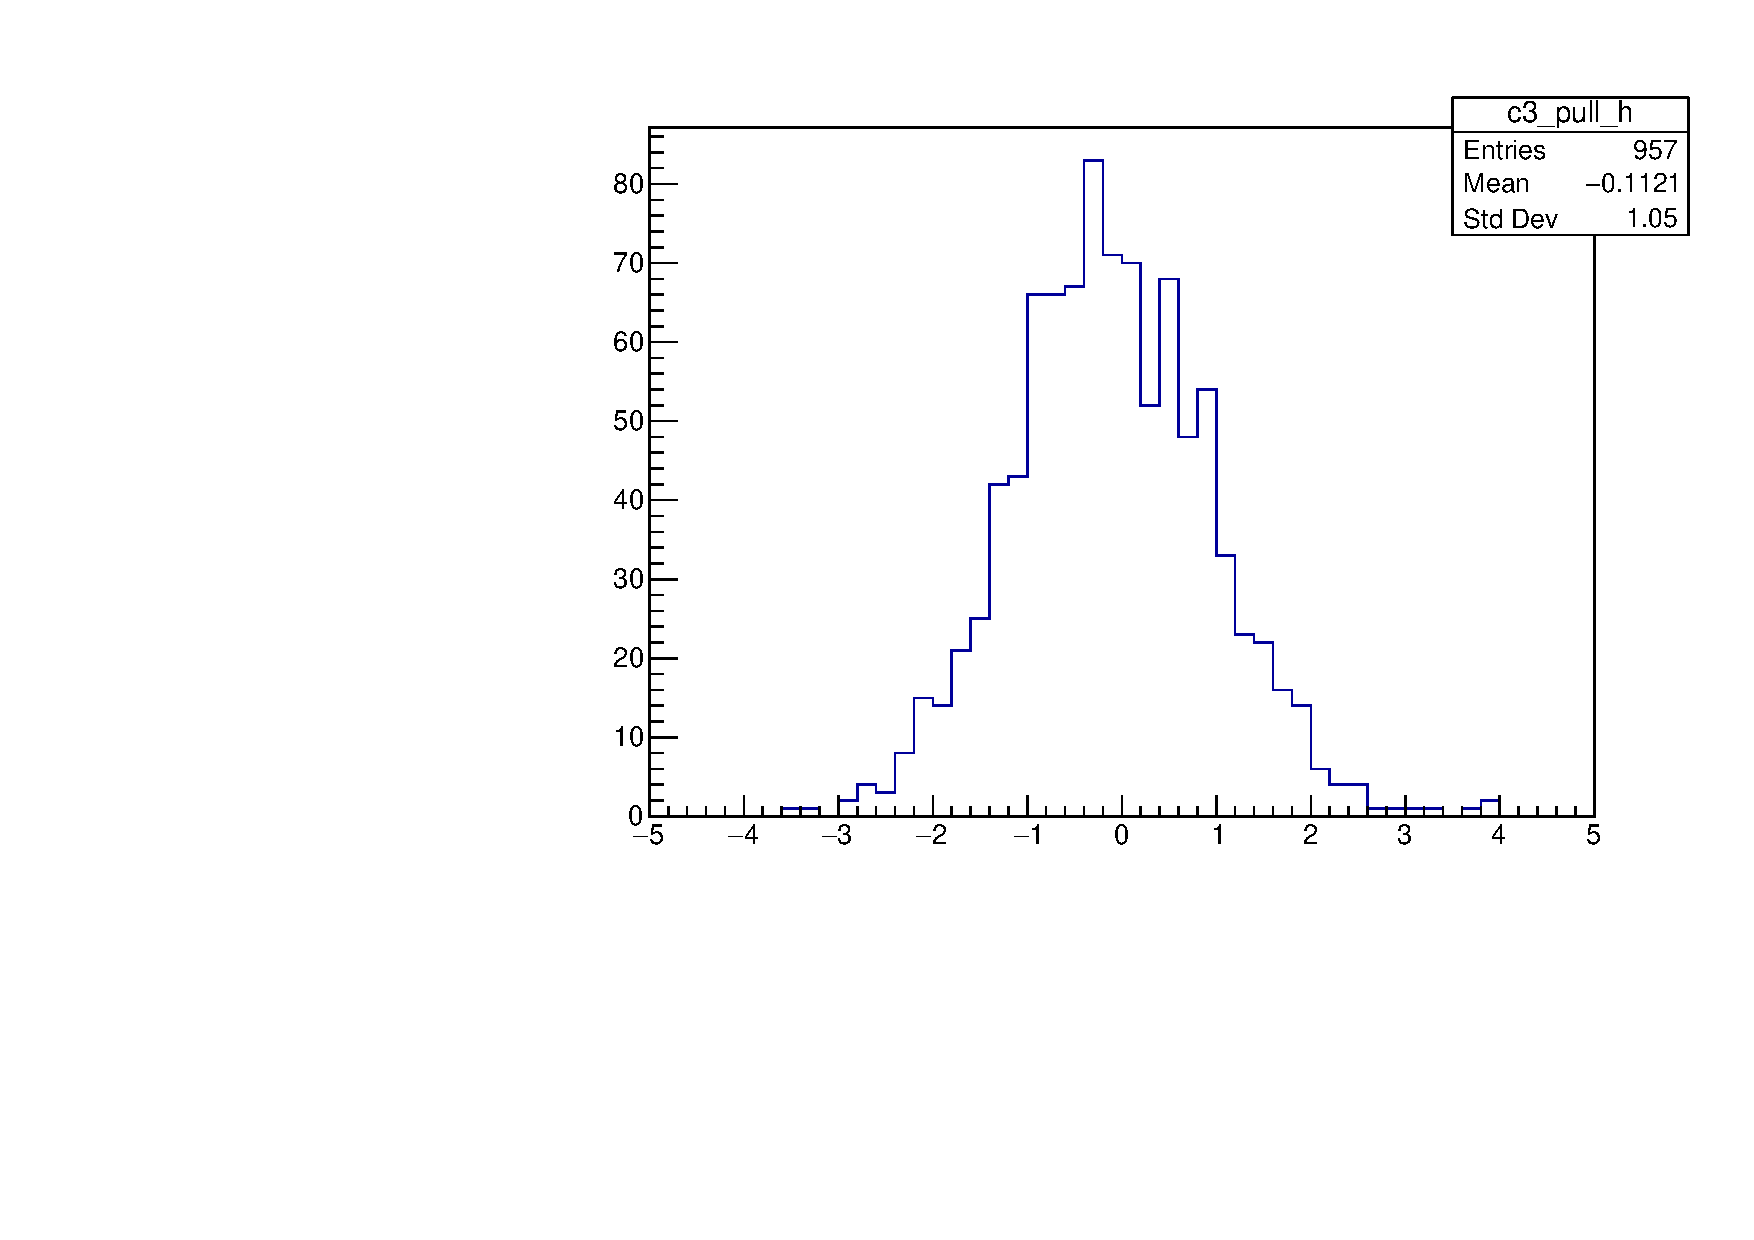
\includegraphics[width=0.75\textwidth,trim={0 0 0 0},clip=true]{Plots/c3_ToyFits_pull.pdf}
      \caption{$c_3$ pulls}
    \end{subfigure}%
    \begin{subfigure}{0.5\textwidth}
      \centering
      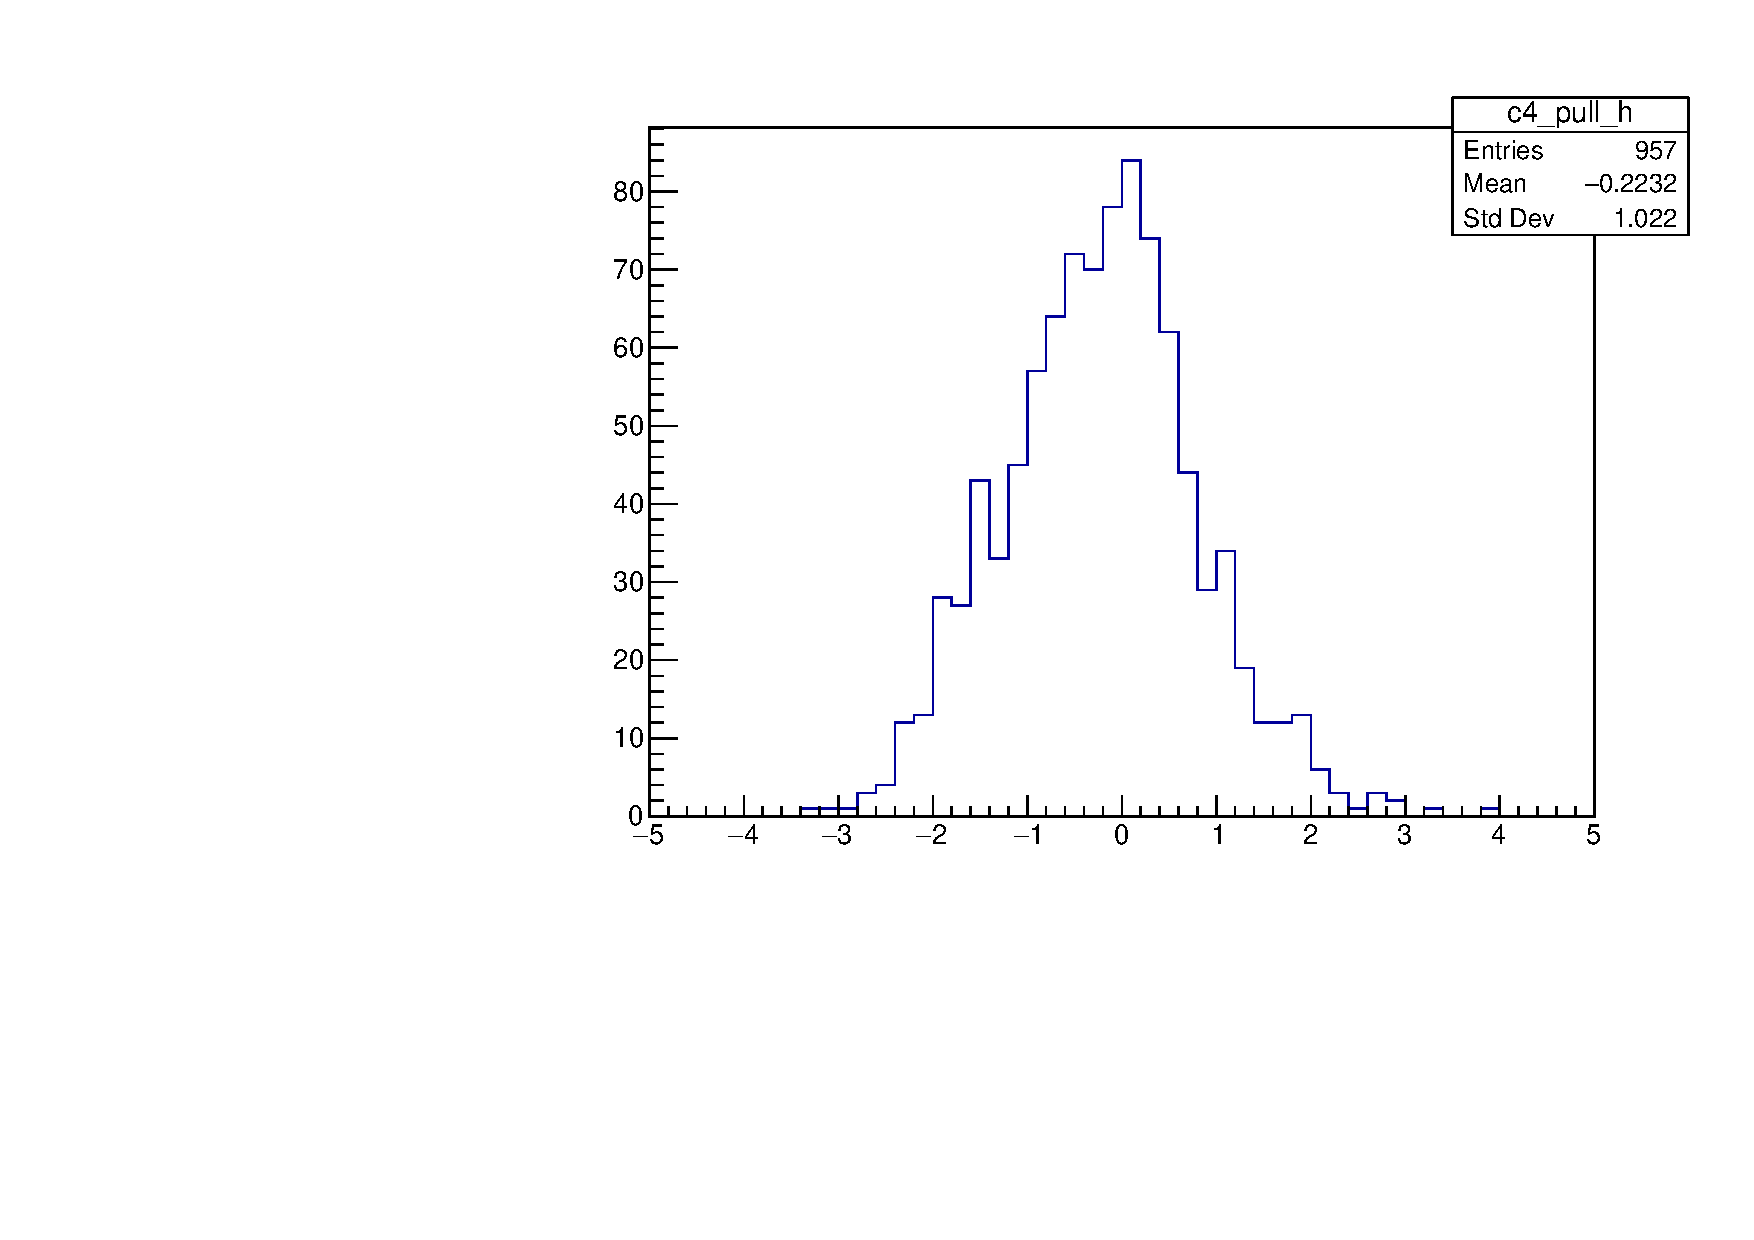
\includegraphics[width=0.75\textwidth,trim={0 0 0 0},clip=true]{Plots/c4_ToyFits_pull.pdf}
      \caption{$c_4$ pulls}
    \end{subfigure}
  \end{figure}
\end{frame}

\begin{frame}{Toy studies}
  \begin{figure}
    \centering
    \begin{subfigure}{0.5\textwidth}
      \centering
      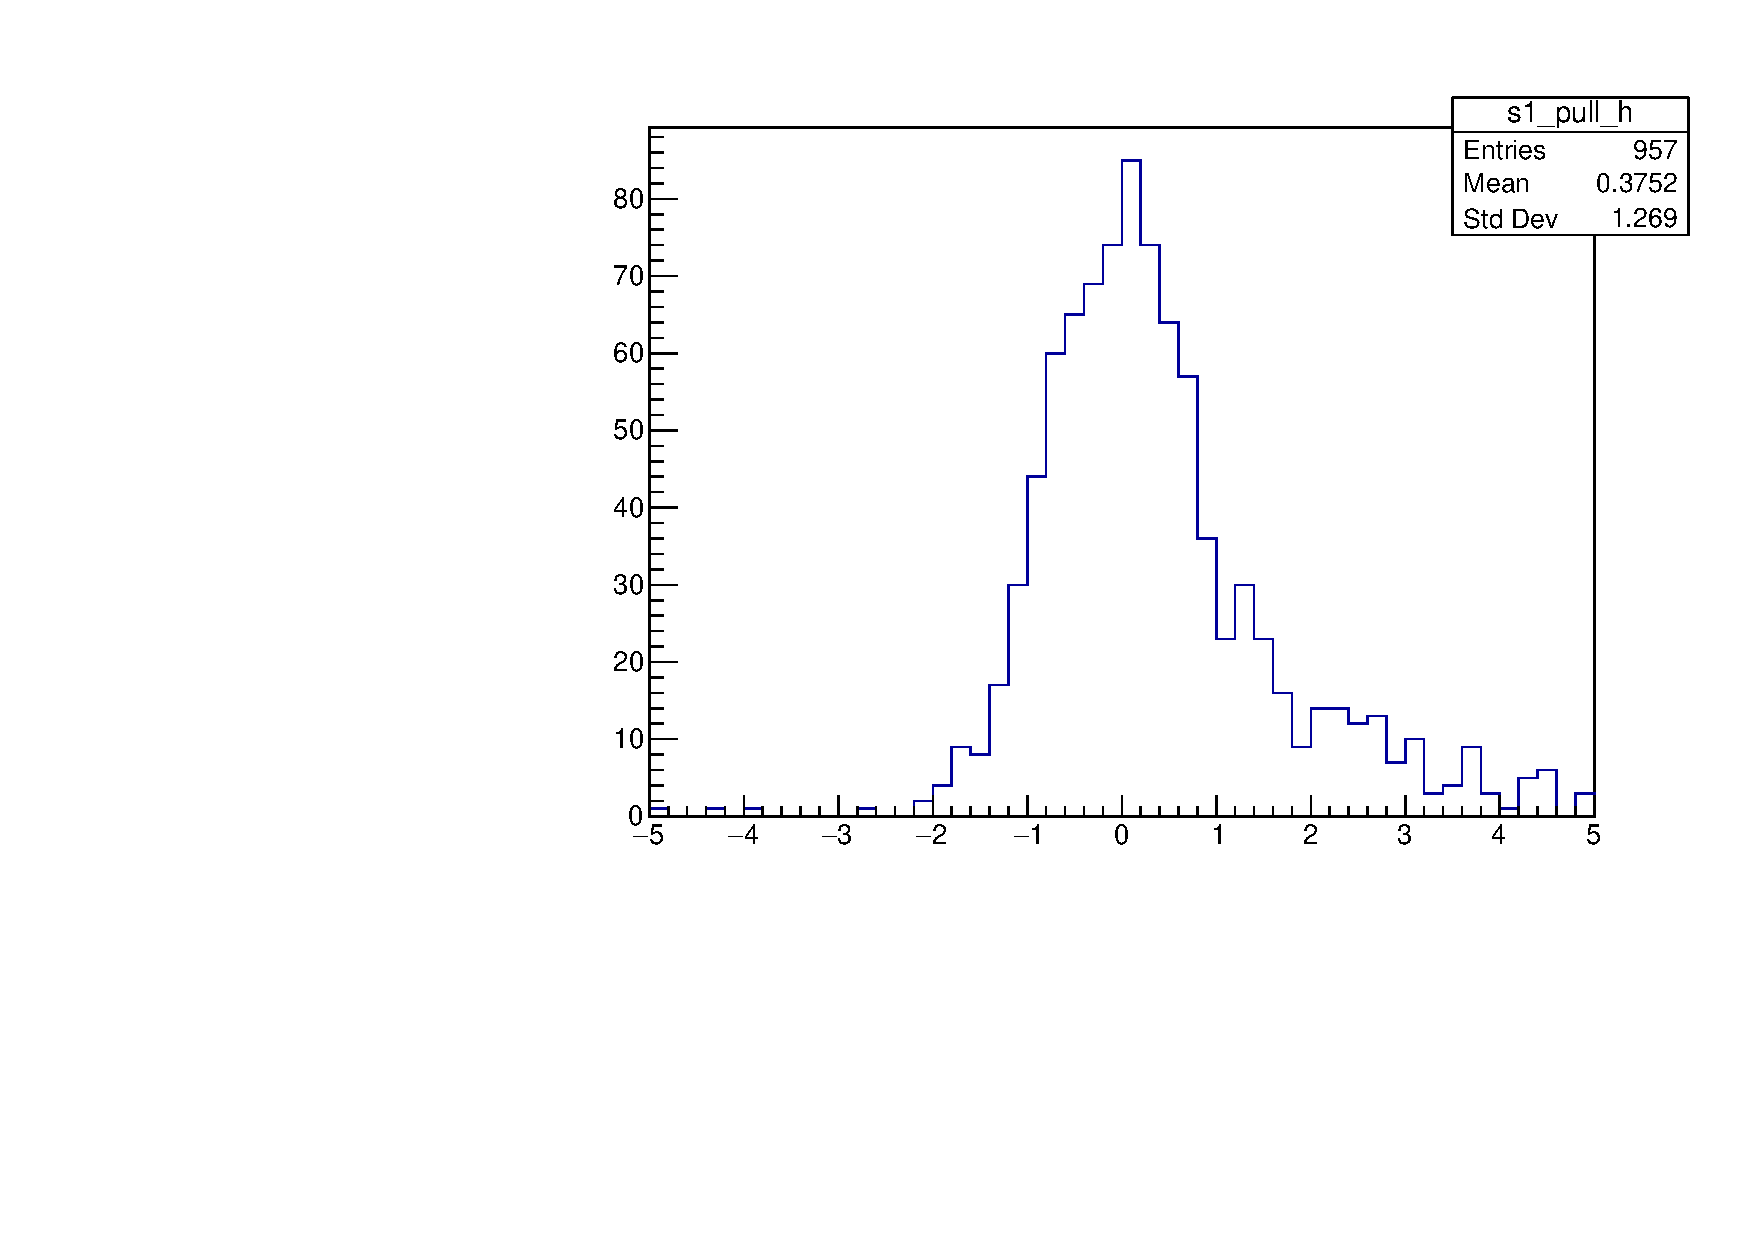
\includegraphics[width=0.75\textwidth]{Plots/s1_ToyFits_pull.pdf}
      \caption{$s_1$ pulls}
    \end{subfigure}%
    \begin{subfigure}{0.5\textwidth}
      \centering
      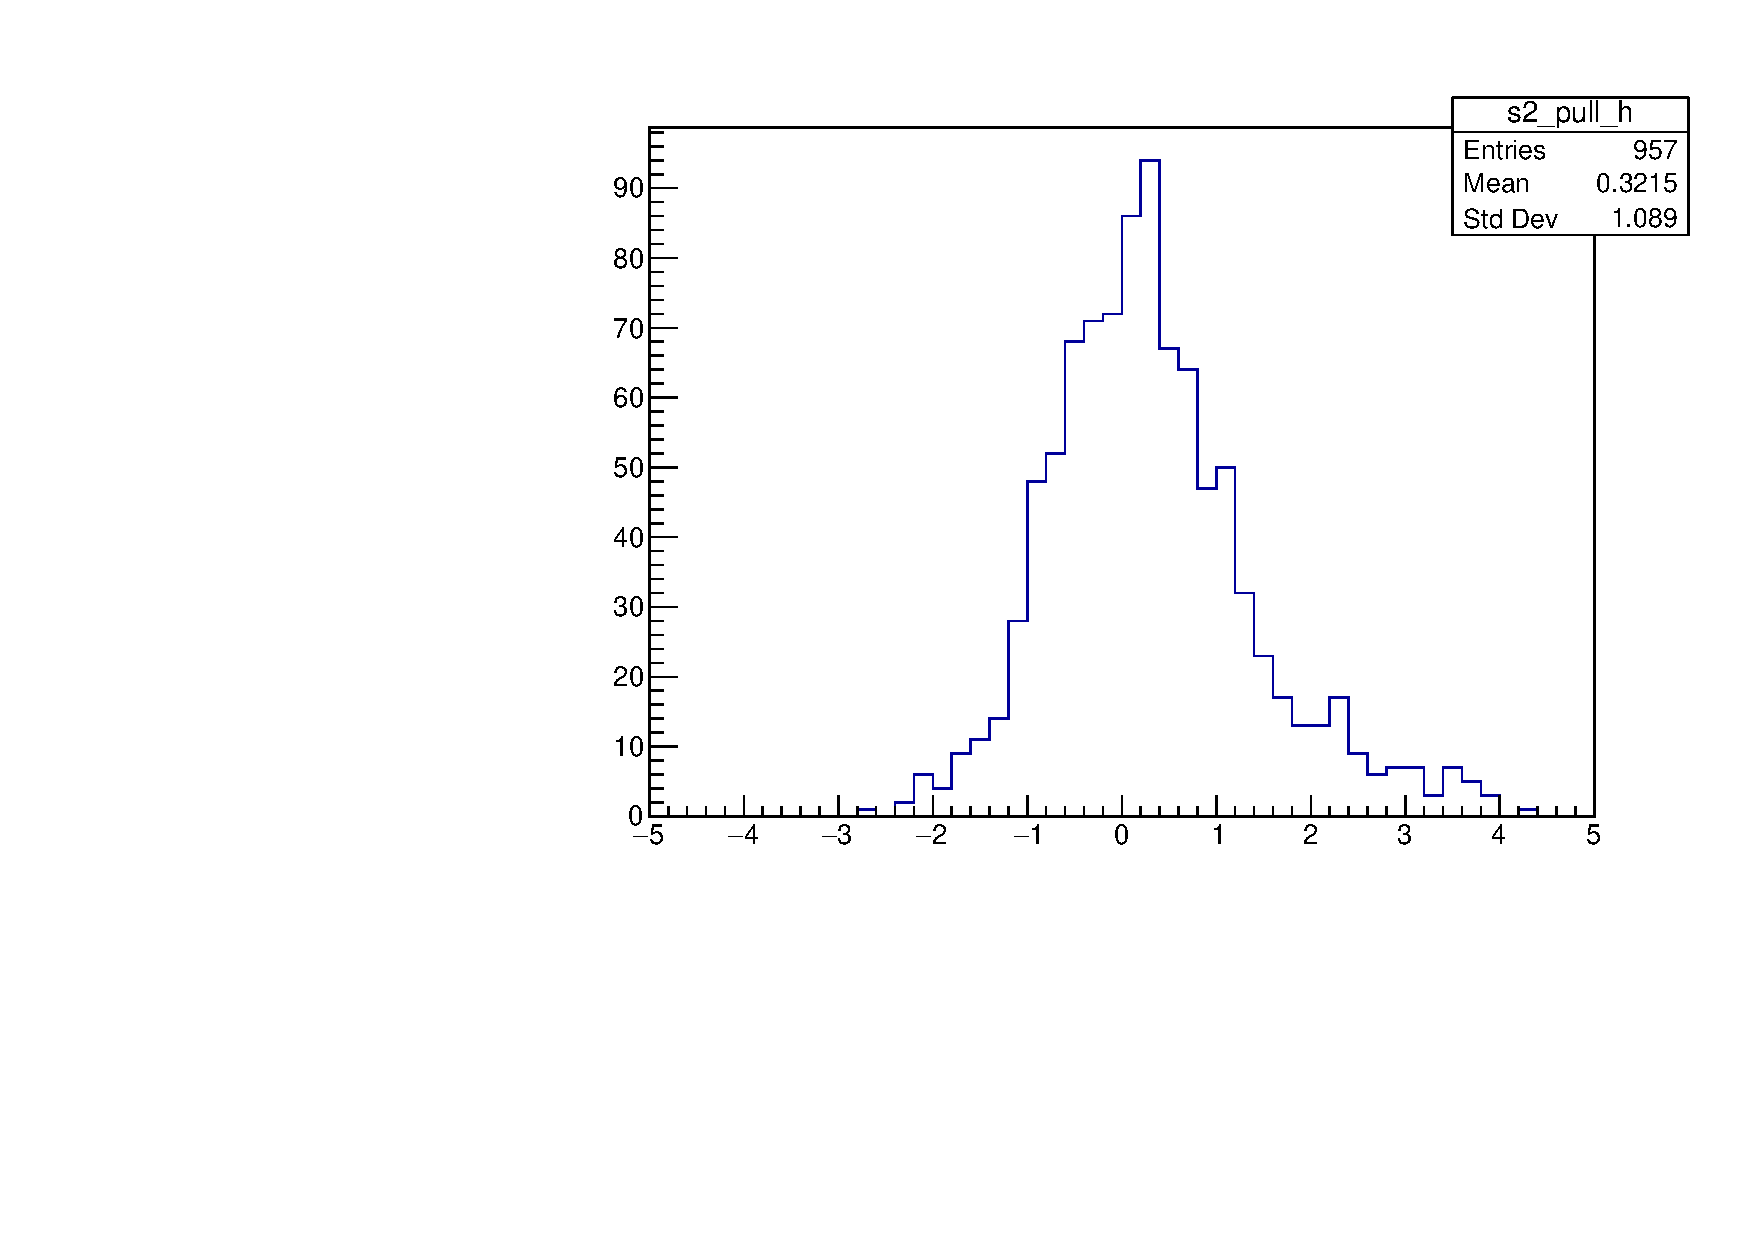
\includegraphics[width=0.75\textwidth]{Plots/s2_ToyFits_pull.pdf}
      \caption{$s_2$ pulls}
    \end{subfigure}
    \begin{subfigure}{0.5\textwidth}
      \centering
      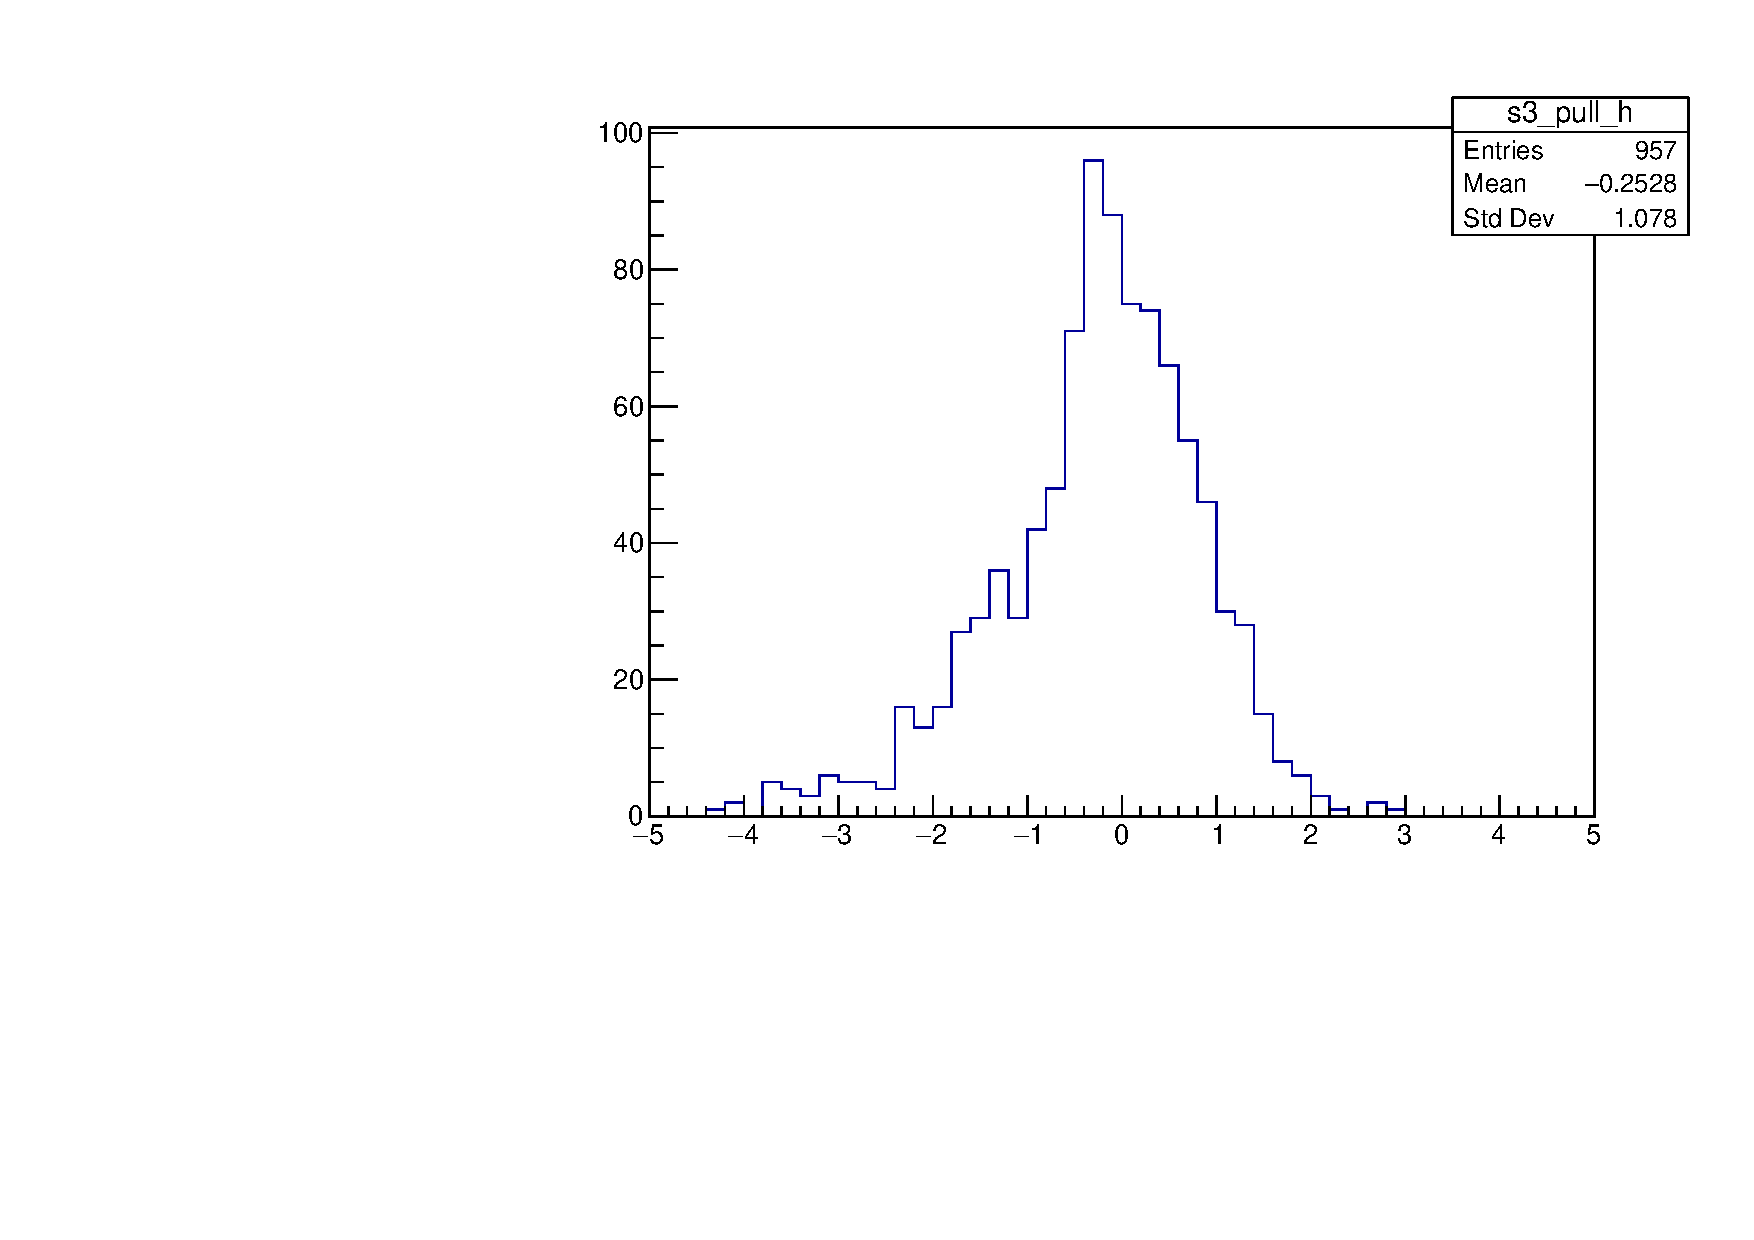
\includegraphics[width=0.75\textwidth]{Plots/s3_ToyFits_pull.pdf}
      \caption{$s_3$ pulls}
    \end{subfigure}%
    \begin{subfigure}{0.5\textwidth}
      \centering
      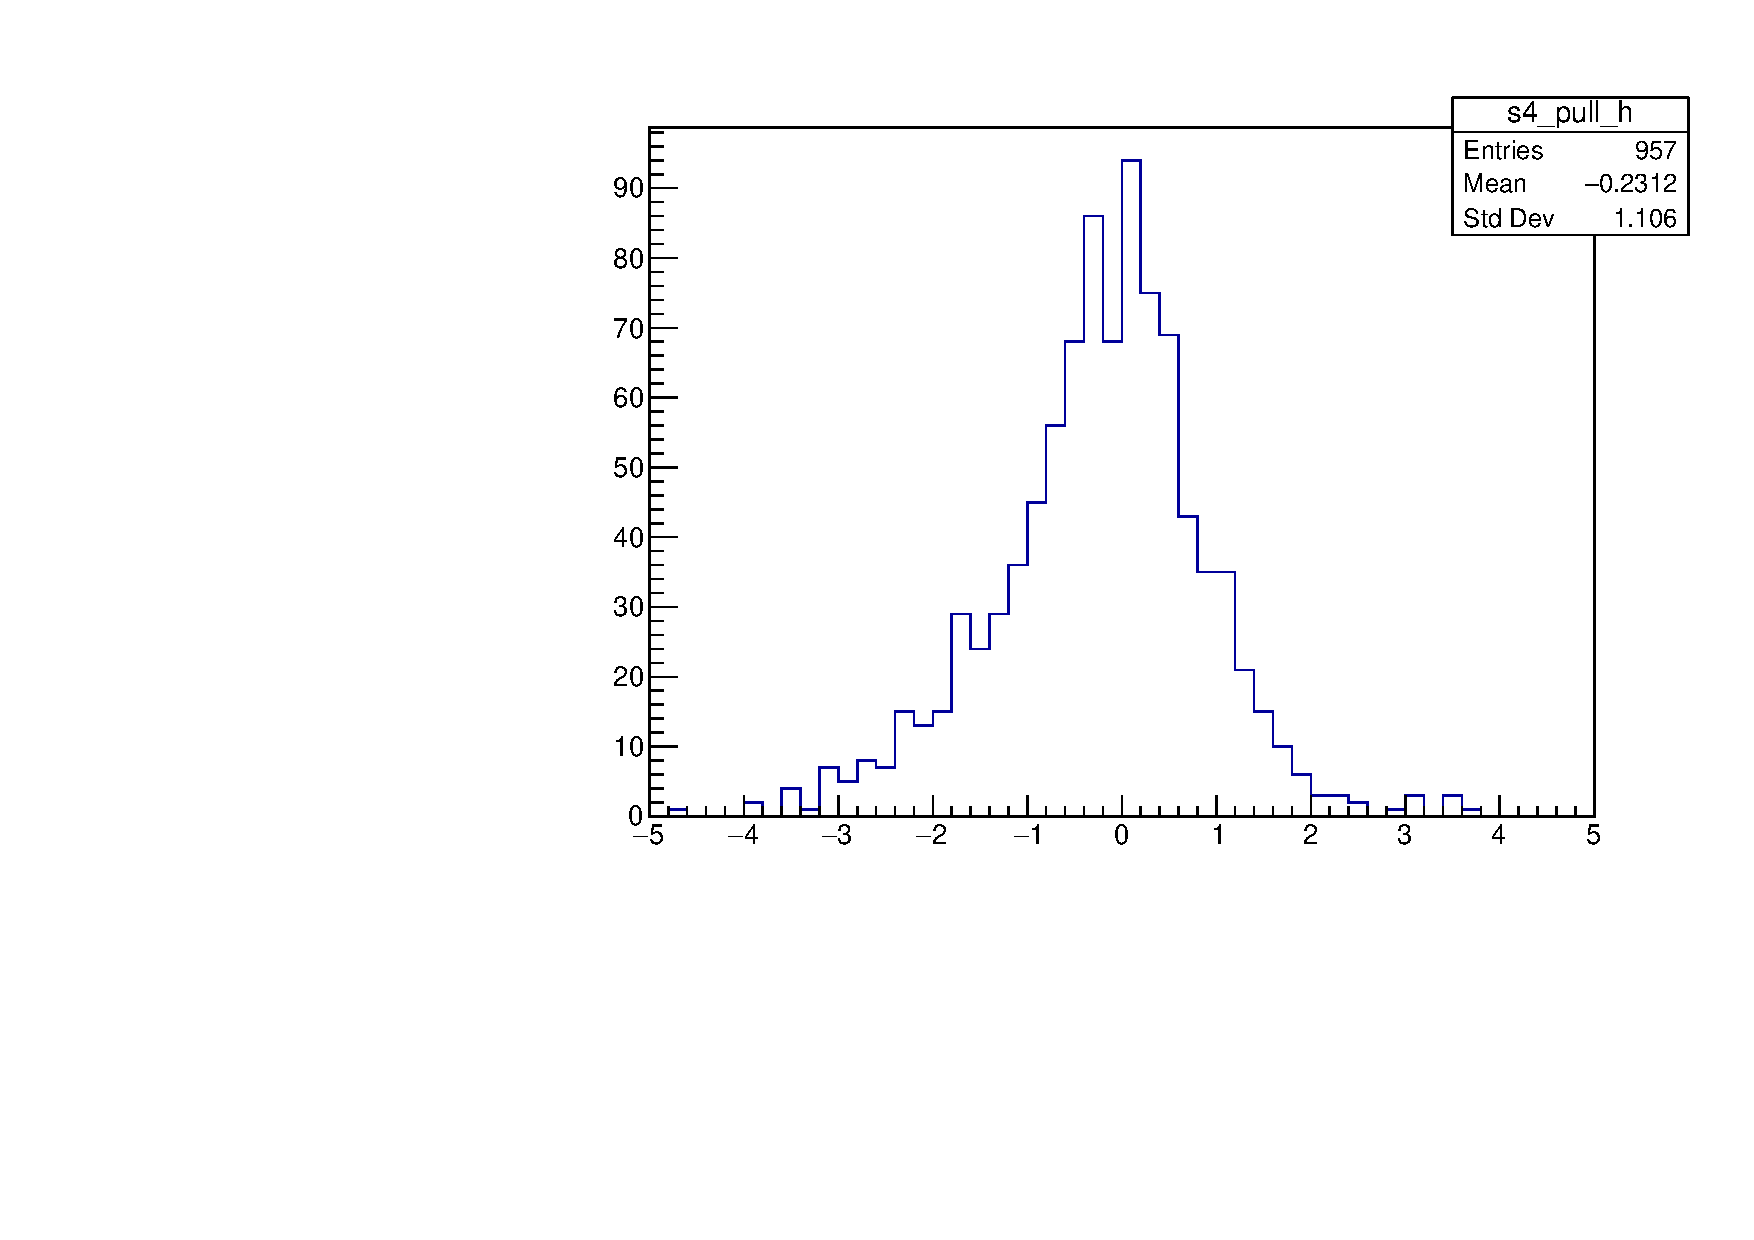
\includegraphics[width=0.75\textwidth]{Plots/s4_ToyFits_pull.pdf}
      \caption{$s_4$ pulls}
    \end{subfigure}
  \end{figure}
\end{frame}

\begin{frame}{Toy studies}
  \vspace{0.0cm}
  {\Large What do the toy fits tell us?}
  \vspace{1.0cm}
  \begin{enumerate}
    \setlength\itemsep{2.0em}
    \item{Small bias in $c_i$ which can be corrected}
    \item{$s_i$ pulls are very asymmetric, and uncertainties are not very reliable}
  \end{enumerate}
\end{frame}

\end{document}